\chapter{Geodynamics GEO3-1313 syllabus (Utrecht University)} %%%%%%%%%%%%%%%%%%%%%%%%%%%%%%%%%%%%%

\begin{flushright} {\tiny {\color{gray} chapter9.tex}} \end{flushright}


\index{contributors}{A. van den Berg}
What follows was written by Arie van den Berg and was/is used as the syllabus for the 
3rd year geodynamics course at Utrecht University. It is reproduced with Arie's permission
and has been slightly modified by me.

\section{Introduction} %------------------------------------------------------------------------
The internal constitution of the Earth has been investigated 
systematically from the nineteenth century on.
With the advent of seismological instrumentation for
the registration of tele-seismic events,
by the end of that century, the main tool for
obtaining direct information about distribution of the material 
properties controling seismic wave propagation became available.
Before this, mainly global properties could be determined from
gravity and magnetic field observations, astronomical data and 
indications about the heatflow from the Earth's interior.
As a result of the early seismological investigations the
main internal structure of the Earth was revealed within the 
first few decades of the twentieth century with the discovery of the
earth's core in 1906 by Oldham and Gutenberg (1912) and the solid 
inner core in 1936 by Lehmann. 

From the radial distribution of the seismic velocity profile, 
obtained by processing the tables of 
traveltime versus epicentral distance, Williamson and Adams (1923) \cite{wiad23}
made a first estimate of the density profile for a compressible
homogeneous mantle model,
consistent with the total mass of the Earth
and obtained at the same time strong indication 
for a high density core, compositionally distinct from the mantle.
They concluded that "It is therefore impossible to explain the high density of the Earth 
on the basis of compression alone. The dense interior cannot consist of ordinary rocks 
compressed to a small volume; we must therefore fall back on the only reasonable alternative, 
namely, the presence of a heavier material, presumably some metal, which, 
to judge from its abundance in the Earth's crust, in meteorites and in the Sun, is probably iron."
 
Bullen\footnote{Keith Edward Bullen (29 June 1906 – 23 September 1976) was a 
New Zealand-born mathematician and geophysicist. He is noted for his seismological interpretation of 
the deep structure of the Earth's mantle and core.} (1975) \cite{bull75} 
further refined the analysis and showed the assumption 
of a homogeneous mantle to be inconsistent with the known moment of 
inertia of the Earth.
In the 1940s and 1950s he introduced a global divison of the
Earth in concentric shells, labelled A through G, ranging from the
Earth's crust (A), bounded by the moho discontinuity, 
to the inner core (G).
Region C between, roughly 400km and 900km, characterized by rapid 
increase of the seismic velocities, was identified by Bullen as
a transition region between the upper mantle region B and a
homogeneous lower mantle, region D.
The deduced inhomogeneity of the mantle was projected by Bullen in this
C region. 
E through G were used to label subdivisions of the core.
Region E indicated the liquid, adiabatic outer core,
F a transition region between inner and outer core and G the solid
inner core.
Birch (1952) \cite{birc52} published improved equations of state,
based on finite-strain theory,
thereby giving a more firm physical basis to interpretation of 
available data in terms of a compressible medium.
  
In the second half of the twentieth century the resolution and 
accuracy of the models were further improved using 
continuously improved seismological observations and a growing 
data set.
It also became possible to obtain independent information about
the radial density distribution from spectral analysis of 
radial eigen-vibrations of the Earth after very large earthquakes.
This development resulted in the publication of the 
Preliminary Reference Earth Model (PREM) by Dziewonski and Anderson (1981) \cite{dzan81}
which still serves as a global reference.

%\begin{center}
%\includegraphics[width=8cm,frame]{images/prem1}
%\includegraphics[width=8cm,frame]{images/prem2}\\
%{\small 
%Upper mantle velocities, density and anisotropic parameter $\eta$ in PREM. 
%The dashed lines are the horizontal components of velocity. The solid curves are $\eta$, $\rho$ and the vertical,or radial, components of velocity.}
%\end{center}

The improved seismologial models indicated
that the continuous rapid velocity increase in the transition zone (C) 
was actually a succession of several abrupt changes,
confirming radial inhomogeneity in mineral phase and possibly in 
chemical composition of the mantle.
 
From geological and cosmochemical arguments a probable composition of 
the Earth had been derived consisting of a mantle with major element
composition dominated by magnesium-iron silicates and an iron-nickle
core with a small amount of lighter elements mixed in,
most likely including mainly sulphur. 
In the 1960s this resulted in the definition of a so-called
pyrolitic composition of the mantle by Ringwood
which could explain the main
mantle petrological observations regarding the complementary
nature of basalts and ultra mafic mantle rocks found in ophiolites, 
kimberlites and mantle perioditite bodies
(Ringwood, 1975 \cite{ring75}). 

In experimental high-pressure and temperature work on the 
candidate mantle materials a series of phase transitions were found
at pressure and temperature values relevant for the Earth's mantle
which could be related to the seismic discontinuities 
revealed by the seismological data.
From these the most prominent at approximately 410 and 660 km depth 
were identified as the phase transition of the olivine component 
$\mathrm{(Mg,Fe)_2 SiO_4}$
of the pyrolitic mantle
to a denser wadsleyite crystal structure and,
at 660 km, a transition (dissociation) from a $\gamma$-spinel 
(known as ringwoodite) structure to a two-phase assemblage, 
post-spinel, i.e.
magnesium-iron perovskite, 
$\mathrm{(Mg,Fe)SiO_3}$ and w\"{u}stite $\mathrm{(Mg,Fe)O}$. 

It was also found that the 660 km boundary corresponds to an
endothermic phase transition which would have implications for 
large scale circulation in the mantle, leading to long-standing 
speculations about the degree of layering in mantle convection
(Christensen \& Yuen (1985) \cite{chyu85},
Albarede \& van der Hilst (2002) \cite{alva02}), \url{http://www.mantleplumes.org}.

A more recent development in this area is the discovery of a new phase
transition of magnesium-perovskite to a denser form for pressure
temperature conditions, approximately 125 GPa 2500 K, relevant for the D"
layer close to the core-mantle boundary
(Lay et al., 2005, van der Hilst et al., 2007).

\begin{center}
\includegraphics[width=12cm]{images/gravity/effect}\\
{\captionfont Effect of water on the phase relations in Earth's mantle and deep water cycle,\\
Litasov \& Ohtani (2007) \cite{lioh07}} 
\end{center}


~\\
In the following sections the density distribution in the
Earth's interior is treated in relation to the gravity field
and internal pressure distribution of a self-gravitating compressible
planet model and the link is shown with results from theoretical
mineral physics and high pressure-temperature experimental data for
mantle materials.
 %---------------------------------------------------------------------
\section{Global internal structure and temperature of the Earth} %------------------------------
To understand the Earth's internal dynamics and evolution we need
to know its internal structure and material properties.
What do we know about Earth's global internal structure?

For a substance of given chemical composition, the material properties
are determined by temperature and pressure.
A full understanding of the Earth's internal dynamics therefore
requires that we know the internal distribution of composition, 
temperature and pressure as illustrated in the following figure:

\begin{center}
\includegraphics[width=10cm]{images/gravity/reg}\\
{\captionfont
Illustration of the central roles that pressure, temperature and density play in geophysics.\\ 
Taken from Regenauer-Lieb et al., Phil. Mag., 2006 \cite{rehy06}.
}
\end{center}
 
The internal pressure distribution is directly linked with the Earth's 
own internal gravity field and density distribution because
the local pressure gradient equals the local gravity acceleration
times the density (see problem \ref{problem-pressure}).
In Section~\ref{section_Density-gravity-pressure} density, gravity
and pressure are treated together in a consistent way. 

If the internal pressure distribution is known we can relate sharp
transitions in the physical parameters as shown in the PREM model,
illustrated in the following figure 
to phase transitions, solid-solid or solid-liquid, 
in the Earth's deep interior.

\begin{center}
\includegraphics[width=8cm]{images/gravity/PREM-inc-pressure}\\
{\captionfont Radial (depth)distribution of density $\rho$, 
seismic velocities $v_p$ and $v_s$,
gravity acceleration $g$ and pressure $P$ \\
in the PREM model (Dziewonski and Anderson (1981) \cite{dzan81}).}
\end{center}


Phase transitions in `candidate' materials for the Earth's interior
are investigated under high pressure and temperature conditions in
HPT laboratory experiments
\footnote{
Deep Earth pressure and temperature conditions can be produced in 
a Diamond Anvil Cell (DAC),
see \url{http://en.wikipedia.org/wiki/Diamond\_anvil\_cell}.
}.
Using theoretical mineral physics models the complete mineral phase 
diagram of mantle silicates can, in principle,
be constructed from a limited set of experimental data
(Stixrude \& Lithgow-Bertelloni (2005) \cite{stli05,stli05b}
Jacobs \& de Jong (2007) \cite{jade07}).  
To constrain the possible candidate materials we also need to know 
the internal distribution of the Earth's chemical composition.
Such composition models are derived from geological evidence and
cosmochemical considerations.


Table I of (Dziewonski and Anderson (1981) \cite{dzan81}) gives 
an expression for the density as a function of the radius $r$, which 
I have turned into a python function:
\begin{lstlisting}
def prem_density(radius):
    x=radius/6371.e3
    if radius>6371e3:
       densprem=0
    elif radius<=1221.5e3:
       densprem=13.0885-8.8381*x**2
    elif radius<=3480e3:
       densprem=12.5815-1.2638*x-3.6426*x**2-5.5281*x**3
    elif radius<=3630.e3:
       densprem=7.9565-6.4761*x+5.5283*x**2-3.0807*x**3
    elif radius<=5600.e3:
       densprem=7.9565-6.4761*x+5.5283*x**2-3.0807*x**3
    elif radius<=5701.e3:
       densprem=7.9565-6.4761*x+5.5283*x**2-3.0807*x**3
    elif radius<=5771.e3:
       densprem=5.3197-1.4836*x
    elif radius<=5971.e3:
       densprem=11.2494-8.0298*x
    elif radius<=6151.e3:
       densprem=7.1089-3.8045*x
    elif radius<=6291.e3:
       densprem=2.6910+0.6924*x
    elif radius<=6346.e3:
       densprem=2.6910+0.6924*x
    elif radius<=6356.e3:
       densprem=2.9
    elif radius<=6368.e3:
       densprem=2.6
    else:
       densprem=1.020
    return densprem*1000
\end{lstlisting}

\begin{center}
\includegraphics[width=8cm]{images/prem/rho.pdf}\\
{\captionfont PREM density as computed with the function above. 
Code available in /images/prem/} 
\end{center}


%--------------------------------------------------
\subsubsection{Early models of the Earth's density}

The total Earth mass $M_{\oplus}$ and average density $\left <\rho \right >$
were not known 
before independent measurement of Newton's gravitational 
constant by Cavendish, 
(see Section~\ref{section_Density-gravity-pressure}).
When the average density had been determined as approximately 
$5.5 \cdot 10^3~\mathrm{kg\cdot m}^{-3}$ it became clear, 
from the lower density of surface rocks of around 
$2.7 \cdot 10^3~\mathrm{kg\cdot m}^{-3}$,
that the Earth's interior must consist of higher density material.

Besides the mass or average density the (average) 
moment of inertia $I$ (defined in Section~\ref{sect_scalarmomint}) 
provides a constraint on the radial distribution of density.
     
These two integral parameter values have been applied in several 
two-parameter models for the radial density distribution of the Earth.
At the end of the nineteenth century Wiechert\footnote{Emil Johann 
Wiechert (26 December 1861 – 19 March 1928) was a German physicist 
and geophysicist who made many contributions to both fields, 
including presenting the first verifiable model of a layered structure of the 
Earth and being among the first to discover the electron.} assumed that the 
compressibility of Earth materials would be negligible to first
approximation and that Earth's high mean density was due to a dense,
probably metallic, core.
He assumed an iron core based on astronomical evidence of high iron
content of the sun's outer layers 
(see also Section~\ref{section-chemical-composition}).

Wiechert considered in particular layered spherically symmetric 
models consisting of two uniform layers, core and mantle.
Since the radius of the Earth's core had not yet been determined by
seismology, Wiechert used the core radius $R_c$ and density 
$\rho_c$ as unknown parameters to be determined from the
known data.
Wiechert assumed the density of the mantle to be 
$\rho_m=3.2 \cdot~10^3 \mathrm{kg\cdot m}^{-3}$ and using known values for $M$ and $I$
he derived for the radius of the core
$R_c/R = 0.779$ corresponding to a mantle depth of about
$1400~\mathrm{km}$ and a core density 
$\rho_c=8.2\cdot 10^3~\mathrm{kg\cdot m}^{-3}$.
This model is investigated in problem 
\ref{problem-wiechert-2layermodel}.

Later, after $R_c/R = 0.545$ had been determined using
seismic data, Jeffreys substituted the known value of the
core radius and derived for the mantle and core densities
$\rho_c=12.6\cdot 10^3~ \mathrm{kg\cdot m}^{-3}$ and 
$\rho_m=4.14\cdot 10^3~ \mathrm{kg\cdot m}^{-3}$ (Bullen (1975) \cite{bull75}).
This model is investigated in problem 
\ref{problem-jeffreys-2layermodel}.

The (radially averaged) density distribution in the Earth remains a topic of research
\cite{kenn98}.
 %--------------------------------------------------------------
\subsection{The moment of inertia of a spherically symmetric density distribution} %------------
\label{sect_scalarmomint} 
The moment of inertia $I$ of a point mass of mass $m$,
with respect to a given rotation axis is defined as $I = m d^2$
where $d$ is the distance from the point mass to the axis.
This quantity relates the angular velocity $\omega$, 
about the rotation axis,
to the angular momentum $J$, of the point mass, in $J = I \omega$.
This is an analogous relation as the one between the linear momentum $p$
and the linear velocity $v$, $p = m v$. 
For an extended mass distribution in a volume $V$,
a moment of inertia tensor, $I_{ij}$,
relating the angular momentum vector ${\bf J}$ to the rotation vector ${\bf \Omega}$
can be defined as $J_i = I_{ij} \Omega_j$, where the summation convention for repeated
indices is implied.
This tensor is described by a $3 \times 3$ matrix defined by volume integration
over point masses in the volume.
Here we only consider spherically symmetric mass distributions where
the moment tensor is isotopric, $I_{ij} = I \delta_{ij}$,
with scalar coefficient $I$.
\footnote{
$\delta_{ij}$ is the Kronecker delta, i.e. $\delta_{ij}=1$ for
$i=j$ and zero otherwise. }
In simple terms, the moment of inertia is the same for any rotation axis
through the centre of the spherically symmetric body.

The moment of inertia $I$ can be determined from Earth's global gravity
field and the precession rate of the rotation axis determined 
from astronomical data, see Bullen, {\it The Earth's density}, 1975.
The principal moments of inertia can also be calculated with the hydrostatic
equilibrium figure of the Earth \cite{lihz17}.


The scalar moment of inertia is defined as
a volume integral over point masses,
\begin{mdframed}[backgroundcolor=blue!5]
\begin{equation}
I = \int_V \rho(\vec{r}) d(\vec r)^2 dV. \label{eq:momI}
\end{equation}
\end{mdframed}
where $d(\vec r)$ is the distance from point $\vec{r}$ to the rotation axis.

For a {\it spherically symmetric} body of finite volume, 
it is often expressed in terms of the total mass $M$, the outer radius $R$ 
and a prefactor $f$ as,
\begin{equation}
\boxed{    I = f M R^2}
\label{def_momint_prefact}
\end{equation}

\begin{center}
\includegraphics[width=6cm]{images/gravity/moments}\\
{\captionfont Taken from Wikipedia\footnote{\url{https://en.wikipedia.org/wiki/Moment_of_inertia_factor}}}
\end{center}

We have seen that the planetary mass and surface density were used to
constrain models for the interior density distribution.
These models are further constrained by the planets moment of inertia $I$
that can be determined from (satellite) geodetic and astronomical
observations.
For Earth the following values for the total mass and moment of inertia
prefactor have been found,
\begin{eqnarray}
M &=& 5.97 \cdot 10 ^{24}\si{\kilo\gram} \nonumber\\
I &=& 0.3307 M R^2  \si{\kilo\gram\square\metre} \nonumber
\end{eqnarray}
where $R = 6371\si{\kilo\metre}$ is the mean radius.
The observed moment of inertia prefactor $f=0.3307$ is smaller than the 
value $0.4$ for a homogeneous sphere 
(see problem \ref{momint_homogeneous_sphere}), 
%(see \ref{sect_scalarmomint}), 
another indication of mass concentration towards the earth's centre.

\vspace{0.5cm}
\fbox{
\begin{minipage}{0.9\textwidth}
\begin{problem}
 {\small \it
  Derive the following expression for the moment of inertia of a 
  spherically symmetric Earth model with outer radius $R$,
  \begin{equation}
   I = \frac{8 \pi}{3} 
       \int_0^R \rho (r) r^4 dr
  \label{mominert_uniform_sphere}
  \end{equation}
  {\it Hint:} use the symmetry and compute 
  $I = \frac{1}{3} (I_x + I_y + I_z )$,
  where $I_x$ is the moment of inertia with respect to a rotation axis coinciding
  with the $x$-axis.
 }
\end{problem}
\end{minipage}
}

\vspace{0.5cm}
\fbox{
\begin{minipage}{0.9\textwidth}
\begin{problem}
\label{momint_homogeneous_sphere}
{\small \it
  Derive from Eq.~(\ref{mominert_uniform_sphere}) the value of the 
  prefactor $f$ of the moment of inertia for a uniform sphere.
  {\it answer:} $f=2/5$.

In general the moment of inertia prefactor $f$ is an indicator of the
degree of mass concentration towards the centre of a spherically 
symmetric mass distribution. 
Endmembers of mass concentration are 
a) a concentrated central point mass and 
b) all mass concentrated on a spherical surface of zero thickness.

   Verify that the moment of inertia of the point mass endmember 
   equals zero
   and that for the prefactor for a spherical shell of vanishing thickness 
   we have $f=\frac{2}{3}$. 
}
\end{problem}
\end{minipage}
}

\todo[inline]{Add bit of theory for delta function is sph coords}

\vspace{0.5cm}

Wiechert's two-layer model with a distinct core is constrained 
by the moment of inertia prefactor $f$, the mantle radius $R$ and 
density $\rho_m$
and the total mass $M$ or, equivalently, 
the mean density $\left < \rho \right >$.
Expressions for the core radius $R_c$ and density $\rho_c$   
can be formulated for this model as specified in the following exercise 
(Bullen, 1975).

\todo[inline]{for 2025: add figure for pb 2,3. Add plot of rho(r) for pb 3. }


\vspace{0.5cm}
\fbox{
\begin{minipage}{0.9\textwidth}
\begin{problem}
\label{problem-wiechert-2layermodel}
 {\small \it
  Derive a 2-parameter model for the earth's 1-D radial density 
  distribution $\rho(r)$ consisting of two uniform layers
  (core and mantle) of radius $R_c$ and $R$ respectively and
  with contrasting uniform densities $\rho_c$ and $\rho_m$ for 
  core and mantle respectively.
  Assume $\rho_m$ to be known, leaving $\rho_c$ and $R_c$ as
  unknown parameters that can be determined from the known 
  moment of inertia prefactor $f$ and the average density 
   $\left <\rho \right >$. 

Compute the total mass M

Compute the average density and arrive at:

\begin{equation} 
\left < \rho \right > = \frac{3}{R^3} \int_0^R \rho(r) r^2 dr
\end{equation} 

Use $I=fMR^2$ and the total mass to arrive at:
  \begin{equation} 
    f R^5 \left < \rho \right > = 2 \int_0^R \rho(r) r^4 dr
  \end{equation} 



  Derive the following expressions for $R_c$ and $\rho_c$,
  \begin{equation} 
     \frac{R_c}{R}
       =
     \left (
       \frac{\frac{5}{2}f \frac{\left < \rho \right >}{\rho_m} -1}
            { \frac{\left <\rho \right >}{\rho_m} -1}
    \right )^{1/2}
    ~,~~
     \rho_c = 
        \rho_m 
        \left \{ 1 + 
                 \left ( \frac{R}{R_c} \right )^3 
                 \left ( \frac{\left < \rho \right >}{\rho_m} -1 \right ) 
       \right \}
%%   \rho_c = \rho_m + \left ( \frac{R_c}{R} \right )^{-3}
%%            \left ( \frac{<\rho >}{\rho_m} -1 \right )
  \end{equation} 



 }



\end{problem}
\end{minipage}
}

\vspace{0.5cm}

In Bullen's two-layer model the core radius is assumed to be known
from seismology.
For this model the mantle and core densities can be expressed in the
known parameters in the following problem.


\vspace{0.5cm}
\fbox{
\begin{minipage}{0.9\textwidth}
\begin{problem}
\label{problem-jeffreys-2layermodel}
 {\small \it
  Assume the core radius $R_c$ to be a known parameter in the 
  following.
  Derive a 2-parameter model for the earth's 1-D radial density 
  distribution $\rho(r)$ consisting of two uniform layers
  (core and mantle), with a core and mantle radius $R_c$ and $R$ and
  different uniform densities $\rho_m$ and $\rho_c$ for 
  mantle and core.
  Express the parameters $\rho_m$ and $\rho_c$ in terms of the
  mass and moment of inertia.

  {\it Hint:} compute $M$ first, then $I$, as a function of all other parameters.
  Establish a relationship of the form $(M,I)^T={ A}\cdot (\rho_c,\rho_m)^T$ where
  $A$ is a $2\times2$ matrix.

  {\it Solution:} in matrix-vector format,
  \begin{equation}
  \label{matvec-density-expr-dim}
    \left (
        \begin{array}{c}
               \rho_c \\
               \rho_m \\
        \end{array}
   \right )
   =
   \frac{4\pi}{3\Delta}
    \left (
        \begin{array}{cc}
               \frac{2}{5}(R^5-R_c^5) & -(R^3-R_c^3) \\
              -\frac{2}{5}R_c^5       & R_c^3        \\
        \end{array}
   \right )
    \left (
        \begin{array}{c}
                   M \\
                   I \\
        \end{array}
   \right )
  \end{equation}
  where the determinant 
     $\Delta = \frac{32\pi^2}{45} 
               \left (
                 R_c^3 (R^5 -R_c^5) - R_c^5 (R^3-R_c^3)
              \right ) $.
 }
\end{problem}
\end{minipage}
}

\vspace{0.5cm}

\todo[inline]{Carry out live demo of python code. Code is in images/geodynamics}



\vspace{0.5cm}
\fbox{
\begin{minipage}{0.9\textwidth}
\begin{problem}
SKIP THIS PROBLEM.
{\small \it
The numerical value of the interim expressions in 
(\ref{matvec-density-expr-dim}) exceeds the magnitude of 
single precision real type variables in computer programs,
that are limitid to approximately $1.7 \cdot 10^{38}$.
A work around for this problem may be to use double precision 
real variables that have a higher maximum magnitude
of about $10^{308}$.

An alternative solution is to switch to using non-dimensional 
parameters, denoted by primes, in the following way:
define 
$R_c^{'} =R_c/R$,
$M_0= 4/3 \cdot \pi R^3 \rho_0 $ and %$M^{'}=1$.
$M= M_0 \cdot M/M_0 = M_0 \cdot M^{'}$,
$\rho_c=\rho_0 \rho_c^{'}$,
$\rho_m=\rho_0 \rho_m^{'}$ and express the moment of inertia 
in the reference density $\rho_0$ and outer radius as,
$I = f M R^2= f 4/3\cdot \pi R^5 \rho_0 $.
With these definitions rewrite (\ref{matvec-density-expr-dim}) 
into the non-dimensional form,
  \begin{equation}
  \label{matvec-density-expr-nondim}
    \left (
        \begin{array}{c}
               \rho_c^{'} \\
               \rho_m^{'} \\
        \end{array}
   \right )
   =
   \frac{16\pi^2}{9\Delta^{'}}
    \left (
        \begin{array}{cc}
               \frac{2}{5}(1-R_c^{'5}) & -(1-R_c^{'3}) \\
              -\frac{2}{5}R_c^{'5}     & R_c^{'3}      \\
        \end{array}
   \right )
    \left (
        \begin{array}{c}
                   M^{'} \\
                   f \\
        \end{array}
   \right )
  \end{equation}
  where the determinant 
     $\Delta^{'} = \frac{32\pi^2}{45} 
               \left (
                 R_c^{'3} (1 -R_c^{'5}) - R_c^{'5} (1-R_c^{'3})
              \right ) $.
 }
\end{problem}
\end{minipage}
}

\vspace{0.5cm}

%%\begin{problem}
%%  Show that the moment of inertia can be split in separate contributions
%%  from the mantle and the core, $I = I_m + I_c$.
%%
%%  Derive expressions for $I_m$ and $I_c$ for the above model with uniform 
%%  mantle and core in terms of the masses of equivalent spheres with
%%  radius $R$ and $R_c$ and densities $\rho_m, \rho_c$ and 
%%  the density contrast
%%  $\Delta \rho = \rho_c - \rho_m$.
%%
%%  Show from these expressions that the moment of inertia prefactor $f$
%%  of the two-layer model is smaller or greater than 0.4 in cases where
%%  $\Delta \rho$ is positive or negative respectively.
%%  \newline
%%  {\it Hint:}
%%  Derive an expression for the prefactor $f$ in terms of $\Delta \rho$.
%%\end{problem}

 %------------------------------------

\newpage
\subsection{Density, gravity and pressure in the Earth} %---------------------------------------
\label{section_Density-gravity-pressure} In the Earth's mantle major solid state phase transitions occur in the 
silicate material which constitutes the planetary mantle
outside the metallic iron/nickle core.
These phase transitions are induced by the increase in the static
pressure from a 1 bar ($10^5\si{\pascal}$) atmospheric value at the Earth's surface to 
$136 \cdot 10^9\si{\pascal}$ at the core mantle boundary at a depth of
approximately 2900\si{\kilo\metre}.
Phase transitions in the Earth's interior are associated with changes 
in the elastic wave velocities that can be deduced from seismological 
observations.
In high pressure experiments, phase transitions in candidate mantle
silicates can be studied and correlated with the seismological data
to constrain the mineralogy and pressure/temperature distribution 
in the mantle.
Knowledge of the internal material constitution of the Earth,
such as the mineral phase,
is a requirement for understanding the main geodynamical processes that determine
Earth's evolution.

Density and pressure inside the Earth are linked with self-gravitation.
This means that the hydrostatic or lithostatic pressure is a direct 
result of the gravity field generated by the Earth's own mass 
distribution.
The lithostatic pressure can be expressed as the weight of a column
of unit cross-sectional area extending from zero depth, at the Earth's 
surface, to the depth $z$ of the evaluation point,
\begin{equation}
 P(z) = \int_0^z \rho(z') g(z') dz'
\label{def_pressure_integ}
\end{equation}
where $\rho$ is the mass density and $g$ is the magnitude of
the gravitational acceleration.

The gravity field defining $g$ is generated by the Earth's own density 
distribution.
Weak periodic gravity `perturbations' are generated by celestial
bodies, expressed in the external tides, both ocean tides and solid
earth tides.
The main tides are generated by the Earth's moon and by the Sun.

In the following section expressions for the gravity field in terms
of the density distribution are given, based on Newton's law of
gravitation.

In the description of the density distribution we will first neglect 
the role of self-compression and consider a number of one-dimensional 
(1-D), spherically symmetric, parameterized density distributions.
Self-compression and compressibility are then treated in section 
\ref{Pressure_density}.
Self-compression and finite compressibility result in a 
continuous increase of density with pressure in agreement 
with several geophysical observations.  

\vspace{0.5cm}
\fbox{
\begin{minipage}{0.9\textwidth}
\begin{problem}
\label{problem-pressure}
 {\small \it
  Derive the expression (\ref{def_pressure_integ}) 
  (where the depth $z$ is not to be confused with a 
   cartesian coordinate)
  for the lithostatic 
  pressure in a spherically
  symmetric planet from the elastostatic equation for a static medium,
  \begin{equation} 
     \partial_j \sigma_{ij} + \rho g_i = 0
\qquad
\Leftrightarrow
\qquad
\vec\nabla\cdot{\bm \sigma} + \rho \vec{g} = \vec{0}
  \label{elastostatic-eqn}
  \end{equation} 
  {\it Hint:}
  Assume hydrostatic conditions where the stress tensor 
  can be written as
  $\sigma_{ij}=-P\delta_{ij}$,
  with $\delta_{ij}$ the Kronecker delta,
  and derive from equation (\ref{elastostatic-eqn})
  for the pressure gradient, $\vec\nabla P = \rho {\vec g}$. 
 }
\end{problem}
\end{minipage}
}

\vspace{0.5cm}

%---------------------------------------------------------
\subsubsection{Gravity field of a mass distribution}
Newton formulated the attraction force acting on a point 
mass $m_0$,  located in a point with position vector ${\vec r}=(x,y,z)$,
with $x,y,z$ the cartesian coordinates,
from a second point mass $m_1$ located at
${\vec r}_1=(x_1,y_1,z_1)$, illustrated in the following figure as,
\begin{equation}
{\vec F} ({\vec r}) 
=\frac{{\cal G} m_0 m_1}{\left | {\vec r}_1 - {\vec r} \right | ^2} ~ 
          {\vec e}_{\vec{r} \vec{r}_1}
\label{pointmass_gravity}
\end{equation}

\begin{center}
\includegraphics[width=7cm]{images/gravity/gravity_diagram}\\
{\captionfont Vector diagram of the gravitational forces acting on the two 
point masses $m_0$, $m_1$ in vector locations ${\vec r}$ and
${\vec r}_1$ respectively.
From the expression for the gravity field (\ref{pointmass_gravity}) 
it follows that the forces on both masses
are of equal magnitude and in opposite direction.}
\end{center}

Where ${\vec e}_{\vec{r}\vec{r}_1}$ is the unit vector in 
${\vec r}$ pointing towards ${\vec r}_1$
and ${\vec F}({\vec r}_1) = - {\vec F}({\vec r})$.
${\vec r}, {\vec r}_1$ 
are the position vectors of the two point masses
and 
$\left | {\vec r}_1 - {\vec r} \right | =
\sqrt{(x_1-x)^2 + (y_1-y)^2 + (z_1-z)^2}$
is the distance between the points ${\vec r}$ and ${\vec r}_1$.
${\cal G}$ is the gravitational constant 
${\cal G} \simeq 6.67 \times 10^{-11} \si{\newton\square\metre\per\square\kilo\gram}$,
$m_0, m_1$ the mass of the respective pointmasses.


This gravitation effect is usually specified as a gravitation force per 
unit mass or acceleration vector ${\vec g}$,
\begin{mdframed}[backgroundcolor=blue!5]
\begin{equation}
{\vec g}({\vec r}) =
\frac{{\cal G} m_1}{\left | {\vec r}_1 - {\vec r} \right | ^2} ~ {\vec e}_{\vec{r}\vec{r}_1} 
\label{grav_accel}
\end{equation}
\end{mdframed}
It can be verified by inspection that the acceleration vector field 
can be written as the 
gradient of a scalar potential field $U({\vec r})$ (i.e. the potential
energy per unit mass) with
\begin{mdframed}[backgroundcolor=blue!5]
\[
{\vec g} = - \vec\nabla U = 
(- \frac{\partial U}{\partial x}, 
 - \frac{\partial U}{\partial y}, 
 - \frac{\partial U}{\partial z}),\]
\end{mdframed}
in Cartesian coordinates (see problem \ref{problem-verify-gradient}),
and
\begin{mdframed}[backgroundcolor=blue!5]
\begin{equation}
U({\vec r}) = - \frac{{\cal G} m_1}{\left | {\vec r}_1 - {\vec r} \right |} 
\label{grav_potential}
\end{equation}
\end{mdframed}

The gravity acceleration and corresponding potential field are additive 
such that the total force or potential of a 
collection of $N$ point masses is obtained by summation over individual
point contributions,
\begin{equation}
{\vec g} ({\vec r}) = 
\sum_j^N \frac{{\cal G} m_j}{\left | {\vec r}_j - {\vec r} \right | ^2} ~ {\vec e}_{\vec{r}\vec{r}_j}
, 
\qquad
U({\vec r}) = 
- \sum_j^N \frac{{\cal G} m_j}{\left | {\vec r}_j - {\vec r} \right |}
\label{eq:gUexo}
\end{equation}
With this definition and sign convention the potential field of
a point source in the origin is represented by a
potential well ($U({\vec r}) < 0$).
This is known as Coulomb's law and the equivalent form for a continuous
mass distribution of density $\rho$ (mass per unit volume) contained in
a volume $V$ is,
\begin{equation}
{\vec g}({\vec r}) = 
\int_V \frac{{\cal G} \rho({\vec r}^{'})}
{\left | {\vec r}^{'} - {\vec r} \right | ^2} ~ 
{\vec e}_{\vec{r}\vec{r}^{'}} ~ dV({\vec r}^{'})
,
\qquad 
U({\vec r}) = 
- \int_V \frac{{\cal G} \rho({\vec r}^{'})}
                     {\left | {\vec r}^{'} - {\vec r} \right |} ~ 
dV({\vec r}^{'})
\label{Coulomb-integrals}
\end{equation}

\vspace{.4cm}

Besides the integral expression for the gravity field defined in
(\ref{Coulomb-integrals}) there is also the differential form
using the second order partial differential equations of Laplace and
Poisson.
It can be shown by verification (see hereafter) that $U$ in (\ref{Coulomb-integrals})
satisfies Poisson's equation, 
\begin{mdframed}[backgroundcolor=blue!5]
\begin{equation}
\vec\nabla^2 U = 4\pi {\cal G}\rho  \label{poisson_eqn}
\end{equation}
\end{mdframed}
which reduces to Laplace's equation $\vec\nabla^2 U = 0$
outside the mass distribution in $V$ (where $\rho =0$). 

To show that $U$ in (\ref{Coulomb-integrals}) satisfies Poisson's
equation integrate the normal component of the acceleration field
over an arbitrary closed surface $S$ enclosing $V$
and change the order of integration for the volume and surface
integral.
\begin{equation}
\int_S \vec\nabla U({\vec r}) \cdot {\vec n} \ dA({\vec r})
   = - \int_V {\cal G} \rho({\vec r}^{'}) 
    \left \{
     \int_S 
       \vec\nabla 
       \left ( \frac{1}{\left | {\vec r}^{'}-{\vec r} \right |} \right )
      \cdot {\vec n} \ dA({\vec r}) 
    \right \} dV({\vec r}^{'})
\label{surface_integral}
\end{equation}
The surface integral on the right is independent of the choice of the
surface $S$ as long as it contains ${\vec r}^{'}$.
We therefore replace this surface by a sphere of radius $R$ centered
at $r^{'}$ and find for the surface integral the value $- 4 \pi$.
\newline
Next we apply the Gauss divergence theorem to the left hand surface 
integral to obtain,
\begin{equation}
\int_V \vec\nabla^2 U \ dV = \int_V 4 \pi {\cal G} \rho \ dV  
\label{int_form_poisson}
\end{equation}
Note that the surface has been contracted on the volume $V$
to obtain (\ref{int_form_poisson}).
Since the surface and enclosed volume are arbitrary we obtain the Poisson
equation,
\begin{equation}
\vec\nabla^2 U  = 4 \pi {\cal G} \rho 
\end{equation}


\vspace{.4cm}

In Newton's time the numerical value of ${\cal G}$ had not been
determined yet. 
As a result it was not possible to determine the mass of the 
Earth $M_{\oplus}$ by measuring the gravitation force of the Earth 
on a known `test mass'.
This way only the value of $G M_{\oplus}$ could be determined.
Only with the experiment named after Cavendish (1798)
\footnote{\url{http://en.wikipedia.org/wiki/Cavendish_experiment}}
it became possible
to measure ${\cal G}$ directly, in a torsion balance experiment,
by determining the gravitational attraction of two closely spaced test 
masses shown here:  

\begin{center}
\includegraphics[width=8cm]{images/gravity/Cavendish_Experiment}
\end{center}

Since Cavendish many experiments have been conducted in order to 
determine the value of this constant:

\begin{center}
\includegraphics[width=9cm]{images/gravity/big_G}\\
{\captionfont This chart compares the results from a dozen experiments measuring ${\cal G}$. 
The vertical stripe represents the most recent recommended value for G (black line) 
with its error bar (gray). Far to the right are the two outlying BIPM measurements, in blue.
Taken from \url{https://www.nist.gov/image/glabel2016plotfromstephanpng}}
\end{center}

The recommended value is ${\cal G}=6.67430(15)\cdot 10^{-11} \si{\cubic\meter\per\kg\per\square\second}$, 
see for instance \url{https://physics.nist.gov/cgi-bin/cuu/Value?bg}.

%---------------------------------------------------------
\subsubsection{Multipole expansion}

The idea behind the multipole expansion is simple: the denominator in Eq.~\eqref{grav_potential}
can be rewritten in such a way that it can be expanded as a Taylor series. 
We have 
\[
\frac{1}{|\vec{r}-\vec{r}'|} 
= \frac{1}{\sqrt{ (\vec{r}-\vec{r}') \cdot (\vec{r}-\vec{r}')   }}
= \frac{1}{\sqrt{ \vec{r}\cdot\vec{r} - 2 \vec{r}\cdot \vec{r}' + \vec{r}'\cdot \vec{r}'   }}
= \frac{1}{r^2} \frac{1}{\sqrt{ 1 - 2 \frac{\vec{r}\cdot \vec{r}'}{r^2} + \left(\frac{r'}{r} \right)^2   }}
\]

The potential can be expanded in a series of Legendre polynomials. 
\[
(1-2XZ+Z^2)^{-1/2} = \sum_{n=0}^\infty Z^n P_n(X)
\]
valid for $|X|\le 1$ and $|Z|\le q$. The coefficients $P_n$ are the Legendre polynomials of degree $n$.


FINISH!

%---------------------------------------------------------
\subsubsection{Gravitational potential energy}


For two pairwise interacting point particles, the gravitational potential energy ${\cal U}$
is given by 
\[
{\cal U} = \frac{-{\cal G} Mm}{R}
\]
where $M$ and $m$ are the masses of the two particles, $R$ is the distance between them.
Close to the Earth's surface, the gravitational field is approximately constant, and the gravitational potential energy of an object reduces to
\[
{\cal U} = m g h 
\]
where $m$ is the object's mass, $g = {\cal G} M_E/ R_E^2$ 
is the gravity of Earth, and $h$ is the height of the object's center of mass above a chosen reference level.







%---------------------------------------------------------
\subsubsection{Let us talk units}
 
The SI units for (gravity) acceleration are $\si{\metre\per\square\second}$.
However in the context of gravity, we will rarely encounter these.

The Gal is the commonly used unit in gravimetry:
\[
0.01 \si{\metre\per\square\second} = 1 {\rm Gal}
\]
and often measurements are given in mGal or $\mu$Gal.

As such, the acceleration due to Earth's gravity 
at its surface is 976 to 983 Gal, the variation being due 
mainly to differences in latitude and elevation. 


%---------------------------------------------------------
\subsubsection{Gravity Force Inside a Spherical Shell}


%from wiki https://en.wikipedia.org/wiki/Shell_theorem

In classical mechanics, the {\it shell theorem} gives 
gravitational simplifications that can be applied to objects inside or outside a 
{\it spherically symmetrical} body. 

Isaac Newton proved the shell theorem and stated that:
\begin{enumerate}
\item A spherically symmetric body affects external objects gravitationally as though all of its mass were concentrated at a point at its centre.
\item If the body is a spherically symmetric shell (i.e., a hollow ball), no net gravitational force is exerted by the shell on any object inside, regardless of the object's location within the shell.
\end{enumerate}

\begin{center}
\includegraphics[width=8cm]{images/gravity/drawing}
\end{center}

These two propositions are not easy to prove. The second one is very important: it states
that if I stand mid-mantle at a radius of, say, 5000\si{\kilo\metre}, the 1371\si{\kilo\metre}-thick 
shell of rock above me does not contribute to the force of gravity that I am feeling. 
Only the rocks below my feet contribute to this force.
At this location we can write
\[
\frac{{\cal G}m M(r)}{r^2} = m a
\]
where $M(r)$ is the mass inside a sphere of radius $r$. The mass $m$ of my body cancels out, and we
obtain 
\[
\frac{{\cal G} M(r)}{r^2} = a
\]
The acceleration in this context is often called $g$ and it clearly depends on $r$ so that 
if density is constant, $M(r)=\frac{4\pi}{3}r^3\rho_0$ and then 
\[
g(r) = {\cal G} \frac{4\pi}{3}r\rho_0
\]
It also follows that the gravity acceleration in the center of the planet ($r=0$) must be zero and 
the gravity acceleration increases linearly with the distance to the center. 
If now the density is not constant (but radially symmetric, i.e. $\rho=\rho(r)$) then 
\[
g(r) =  {\cal G} \frac{4\pi}{r^2} \int_0^r \rho(r') r'^2 dr'
\]
Remember that this is true because of the spherical symmetry!

%---------------------------------------------------------
\subsubsection{Nonuniqueness}

Given a body with mass $M$ at a distance $r$ from me, the gravitational acceleration 
that I feel is 
\[
a = \frac{{\cal G} M}{r^2}
\]
If the mass is now twice as far (distance $2r$) then 
\[
a' = \frac{{\cal G} M}{(2r)^2} =  \frac{1}{4} \frac{{\cal G} M}{r^2} = \frac{1}{4}a
\]
Because of the inverse square of the distance the acceleration is four times as small. 

However, if I now 'make' the mass of the body four times as large and twice as far, 
\[
a'' = \frac{{\cal G} (4M)}{(2r)^2} = \frac{{\cal G} M}{r^2} =a
\]
There lies a very important fact: There is an inescapabale trade-off between distance 
and mass. 

If gravity is measured at a single point in space nothing certain can be said about 
what lies below: the object generating the gravity anomaly could be 'close' and 
not so massive, or 'far' and really massive, 
both situations potentially leading to the same measurement.

\begin{center}
\includegraphics[width=6cm]{images/gravity/nonunique}\\
{\captionfont Taken from \textcite{vapb15} (2015).}
\end{center}


%---------------------------------------------------------
\subsubsection{The Netherlands}

As explained in \textcite{crdv02} (2002),  
in The Netherlands gravity values
increase from south to north with about 1 milligal per kilometer. Smallest values occur
in Limburg (981,100 milligal), while the largest values occur in Groningen (981,350
milligal). Local variations are limited to 1 milligal over some kilometers.


\begin{center}
\includegraphics[height=5cm]{images/gravity/gravityNL}
\includegraphics[height=5cm]{images/gravity/gravityNL2}\\
{\captionfont Left: Taken from \url{https://www.nlog.nl/en/gravity-and-magnetic-field}. 
The size of the Bouguer anomaly at a particular location is a measure of the mass deficit or mass 
excess in the underlying rocks. A mass deficit  exists where  the stratigraphic succession is composed of relatively light rocks; 
this yields a negative Bouguer anomaly. A mass excess exists where the stratigraphic succession is 
composed of relatively heavy rocks, this yields a positive anomaly.
Right: Taken from \url{https://upload.wikimedia.org/wikipedia/commons/c/ce/Valversnelling_in_Nederland.svg}.

}
\end{center}

\begin{center}
\includegraphics[width=8cm]{images/gravity/bodemdaling}\\
{\captionfont Taken from \url{https://bodemdalingskaart.nl/portal/index}. Is the continuous sinking of certain parts of the Netherlands 
visible in the satellite gravity rate measurements ?}
\end{center}

\todo[inline]{write about Anomalies, Additivity, Inversion}



%----------------------------------------------------------------
%\subsubsection{Problem section: spherically symmetric density 
%distributions and corresponding gravity fields}


%---------------------------------------------------------
\subsubsection{A few problems more to solve}

\vspace{0.5cm}
\fbox{
\begin{minipage}{0.9\textwidth}
\begin{problem}
 {\small \it
  Verify that the familiar surface value of the Earth's gravity
  acceleration $g_0=9.8 ~\mathrm{m/s^2}$ corresponds to the value of a point mass
  at the Earth's centre with the same mass as the Earth (see Table).
 }
\end{problem}
\end{minipage}
}

\begin{center}
  \begin{tabular}{|l|c|c|c|} \hline
               & Radius & Mass & Density \\ 
               & km   & kg & $\mathrm{kg/m^3}$\\ \hline
%%%      &             \\
     Earth   & $6371$ & $5.97 \cdot 10^{24}$ & $5.515 \times 10^3$ \\
     Moon    & $1738$ & $7.34 \cdot 10^{22}$ & $3.34  \times 10^3$ \\ 
     Mars    & $3394$ & $6.42 \cdot 10^{23}$ & $3.93  \times 10^3$ \\
     Jupiter &$71492$ & $1.9  \cdot 10^{27}$ & $1.326 \times 10^3$ \\
     Sun     &$6.96\cdot 10^5$ 
                      & $1.99 \cdot 10^{30}$ &        -            \\
%%%      &             \\ 
  \hline
  \end{tabular} \\
{ \captionfont Radius-mass parameters of Earth moon and planets.}
\end{center}


\begin{center}
\includegraphics[width=7cm]{images/gravity/marsgravity}
\includegraphics[width=7cm]{images/gravity/moongravity}\\
{\captionfont Left: Mars gravity, taken from Hirt \etal (2011) \cite{hick12}; 
Right: Moon gravity, taken from \url{https://en.wikipedia.org/wiki/Gravitation_of_the_Moon}}
\end{center}


%REDUNDANT WITH PREVIOUS EX
%\fbox{
%\begin{minipage}{0.9\textwidth}
%\begin{problem}
% {\small \it
%  Compute the Earth's mass $M_{\oplus}$ from the given values of the
%  gravity acceleration at the surface $g_0$, the gravitational constant $G$
%  and the planet radius.
% }
%\end{problem}
%\end{minipage}
%}



\vspace{0.5cm}

\fbox{
\begin{minipage}{0.9\textwidth}
\begin{problem}
 {\small \it
The PREM profile suggests that the magnitude of the gravity aceleration
  is approximately constant throughout the Earth's mantle.
Assume an approximate uniform value of $g$ in the Earth's mantle, equal to the surface value $g_0 \sim 9.8m/s^2$ 
and use an approximate average mantle density $\rho_m\sim 4.5 \times 10^3kg/m^3$ 
to obtain from Eq. (\ref{def_pressure_integ}) an approximation of the static pressure at the core mantle boundary at a depth of 2891km.
 }
\end{problem}
\end{minipage}
}

\vspace{0.5cm}

\vspace{0.5cm}
\fbox{
\begin{minipage}{0.9\textwidth}
\begin{problem}
\label{problem-verify-gradient}
 {\small \it
  Verify the consistency of the expression for the gravity acceleration
  and potential of a point mass in
  (\ref{grav_accel}) and (\ref{grav_potential}),
  i.e. prove from these expressions 
  by explicit calculation of the gradient vector from the
  scalar potential field that ${\vec g}= - \vec\nabla U$.

Hint: specify the potential in \eqref{grav_potential} 
in Cartesian coordinates (i.e. write explicitely $|\vec{r}_1-\vec{r}|$)
and differentiate the result with respect to the coordinates $x,y,z$.
What is the derivative of $(f(x))^\alpha$ with respect to $x$?   
After a few steps you should then arrive at \eqref{grav_accel}. 
 }
\end{problem}
\end{minipage}
}

\vspace{0.5cm}

%%\begin{problem}
%%  The magnitude of the vertical (radial) component of the gravity
%%  acceleration is often expressed as the scalar quantity
%%   $g = \left | g_r \right |
%%      = \left | ( {\bf g} \cdot {\bf e}_r ) \right |$.
%%  \newline
%%  Verify the relation between the magnitude of the vertical 
%%  acceleration and the gravity potential,
%%   \begin{equation}
%%      g = \frac{\partial U}{\partial r}
%%   \end{equation}
%%\end{problem}

%%\begin{problem}
%%  Show by explicit calculation that 
%%  $\nabla \cdot ( 1/r^2 {\bf e}_{\bf r} ) = 0$
%%  and 
%%  $\nabla^2 1/r = 0$ 
%%  outside the origin ${\bf r}=0$. 
%%  In other words, the gravitation force field has zero divergence 
%%  outside it's source, the mass distribution contained in a volume $V$.
%%  Outside $V$ we have $\left | {\bf r}^{'} - {\bf r} \right | > 0$ 
%%  such that we can
%%  differentiate inside the Coulomb integral and obtain 
%%  $\nabla^2 U({\bf r}) = 0$, $( {\bf r} \ni V)$, showing that 
%%  $U$ satisfies the Laplace equation outside $V$.   
%%\end{problem}

\vspace{0.5cm}
\fbox{
\begin{minipage}{0.9\textwidth}
\begin{problem}
 {\small \it
  Apply the Poisson equation (\ref{poisson_eqn}) to obtain the
  gravity field of a 
  point-mass distribution with mass $M$, 
  described by a Dirac delta function, 
  $\rho({\vec r}) = M \delta ({\vec r}-{\vec r}_0)$.
  Where the following property holds for the delta function,
  \begin{equation}
   \int_V \delta( {\vec r}-{\vec r}_0) dV =
     \left \{
       \begin{array}{ll}
         1, ~ {\vec r}_0 \in V \\ 
         0, ~ {\vec r}_0 \ni V \\ 
       \end{array}
     \right .
  ~or,~ more ~general
   \int_V f({\vec r}) \delta( {\vec r}-{\vec r}_0) dV =
     \left \{
       \begin{array}{ll}
         f({\vec r}_0), ~ {\vec r}_0 \in V \\ 
         0, ~ {\vec r}_0 \ni V \\ 
       \end{array}
     \right .
  \end{equation}

  Hint: integrate (\ref{poisson_eqn}) over a spherical volume,
  centered at ${\vec r}_0$ and apply the Gauss divergence theoreme:
  for a vector field ${\vec A}=(A_1,A_2,A_3)$ with divergence 
  $\vec\nabla \cdot {\vec A} = 
   \frac{\partial A_1}{\partial x} +
   \frac{\partial A_2}{\partial y} +
   \frac{\partial A_3}{\partial z}
  $
  \begin{equation}
    \int_{V} \vec\nabla \cdot {\vec A} dV
      =
    \int_{\partial V} {\vec A} \cdot {\vec n} dS
  \end{equation}
  where $\partial V$ is the closed boundary surface of $V$.
 }
\end{problem}
\end{minipage}
}


\vspace{0.5cm}

\fbox{
\begin{minipage}{0.9\textwidth}
\begin{problem}
 {\small \it
  Check the dimensional units in (\ref{poisson_eqn})
  and verify that the gravitational potential has the dimension of 
  energy per unit mass.
  This is in agreement with the identification of the gravity potential
  with the potential (gravitational) energy of a unit mass in the
  gravity field.
\footnote{
  The local potential field value $U({\bf r}_1)$ equals the negative of
  the (gravitational) potential energy $W({\bf r}_1)$ 
  of a unit point mass positioned at ${\bf r}_1$. 
  It can be shown that the change in potential energy $\Delta W$ 
  that results from
  moving a unit mass from ${\bf r}_1$ to ${\bf r}_2$ follows directly
  from the potential field values $U({\bf r}_1)$, $U({\bf r}_2)$ and is
  independent of the path taken between ${\bf r}_1$ and ${\bf r}_2$.
  This property defines a so called conservative field $U$.

  To derive this result we compute the potential energy difference 
  as the path (line) integral of the work done by the gravity force 
  field on a unit mass and apply the gradient property 
  ${\vec g}= - \vec\nabla U$.
The work done by moving a unit point mass from a location
${\bf r}_1$ to
${\bf r}_2$ is defined by the line integral,
\begin{eqnarray}
   \Delta W 
   &=& 
     \int_{{\bf r}_1}^{{\bf r}_2}
               {\bf F} \cdot d{\bf r}
    = 
     \int_{{\bf r}_1}^{{\bf r}_2}
               {\bf g} \cdot d{\bf r}
    = 
     \int_{{\bf r}_1}^{{\bf r}_2}
             - \vec\nabla U \cdot d{\bf r}
    = 
     \int_{U({\bf r}_1)}^{U({\bf r}_2)} - dU
%%%           \nonumber \\
    = 
      -\left ( U({\bf r}_2) - U({\bf r}_1) \right ) = - \Delta U
\label{work-integral}
\end{eqnarray}
Here the following gradient property has been used, 
relating the gradient vector to the differential of the scalar 
potential field,
\begin{equation}
   dU
    =
   \frac{\partial U}{\partial x} dx + 
   \frac{\partial U}{\partial y} dy + 
   \frac{\partial U}{\partial z} dz
    =
   \vec\nabla U \cdot d{\vec r} 
\end{equation}
The gravitational potential field can thus be defined in terms of the
work done by the gravity field to move a unit mass from infinity 
to the evaluation point.
\begin{equation}
   W({\bf r}_1) 
    =
    \int_{{\bf r}_\infty}^{{\bf r}_1}
     {\bf g} \cdot d{\bf r}
    =
    \int_{{\bf r}_\infty}^{{\bf r}_1}
     -\vec\nabla U \cdot d{\bf r}
    =
    \int_{U({\bf r}_\infty)}^{U({\bf r}_1)}
     -dU
    =
     - U({\bf r}_1) + U({\bf r}_\infty) = - U({\bf r}_1)
\end{equation}
Where $U({\bf r}_\infty) = 0$ has been used.
}
 }
\end{problem}
\end{minipage}
}

\vspace{0.5cm}

The above can be applied in the 
determination of the escape velocity from the
surface of a planet. 
This is the minimum launch velocity to escape from the planet's gravity
field. 
For a spherically symmetric planet the external gravity potential is
given by (\ref{grav_field_unif_sphere}).
Moving an object from the surface, the gravity potential changes 
by $\Delta U = U(r) - U(R) = {\cal G} M(-\frac{1}{r} + \frac{1}{R})$.
Applying an energy conservation argument we require the change
in total (potential plus kinetic) energy per unit mass to be:
$\Delta E= \Delta U + \Delta K = 0$. 
With $\Delta K = - v_{ex}^2 /2$ we get $v_{esc} = \sqrt{2{\cal G}M/R}$.

\vspace{0.5cm}
\fbox{
\begin{minipage}{0.9\textwidth}
\begin{problem}
{\small \it
Compute the surface escape velocities for different celestial bodies
using the parameters given in the Table above. 
}
\end{problem}
\end{minipage}
}


\vspace{0.5cm}

To watch: 
\begin{itemize}
\item Tossing Satellites into Orbit with SpinLaunch: Is that Possible? (3min) \\
\url{https://www.youtube.com/watch?v=-BCeanUiKwM}
\item Can We Throw Satellites to Space? (42min) \\
\url{https://www.youtube.com/watch?v=yrc632oilWo}
\end{itemize}

\vspace{0.5cm}


\vspace{0.5cm}
\fbox{
\begin{minipage}{0.9\textwidth}
\begin{problem}
 {\small \it
  The potential energy of a self-gravitating planet in its own
  gravity field is defined 
  in terms of the volume density $\rho U$ as,
  \begin{equation}
     E = - \int_V \rho U dV
  \end{equation}
  Derive the following expression for the potential energy
  of a spherically symmetric, uniform density model,
  using the expression for the internal gravity potential defined in
  (\ref{grav_field_unif_sphere_int})
  \begin{equation}
    E = \frac{8\pi}{5} {\cal G} \rho_0 M R^2
  \end{equation}
  Compute the potential energy value $E$, 
  assuming a density 
   $\rho_0=5.5\cdot 10^3 \mathrm{kg/m^3}$ and planetary radius 
   $R = 6371 \mathrm{km}$.
  \newline
  {\it answer: $4.4 \cdot 10^{32} \mathrm{J}$}
 }
\end{problem}
\end{minipage}
}

\vspace{0.5cm}


The gravitational energy considered above plays an important role
in major compositional differentiation processes that occurred 
in the early Earth and are still occuring today.
\begin{itemize}
\item
  A so called `core catastrophe' occured when
  the iron/nickel core of the Earth differentiated from the silicate mantle
  in the first few million years after the formation of the Earth
  in the early solar system.
  This event has probably freed enough potential energy to melt the mantle 
  completely, resulting in a global magma ocean \footnote{https://en.wikipedia.org/wiki/Iron\_catastrophe}.
\item
  Crystallization of the solid inner core from the liquid outer core,
  as a result of core cooling,
  is accompanied by compositional differentiation. 
  The liquid outer core contains a lighter fraction, possibly sulfur,
  which stays behind in the liquid during freezing of the inner
  core.
  The enriched residual liquid near the inner core boundary is less
  dense than the average liquid of the outer core and this results
  in a gravitationally unstable layering that induces
  `chemically driven' convective flow in the outer core.
  The potential energy released in this chemical convection is 
  probably an important energy source in powering the geodynamo
  that generates the Earth's present day magnetic field.
\end{itemize}
 %----------------------

\subsection{The gravitational potential for spherical problems}

Starting from the Poisson equation, 
\[
\Delta U = 4 \pi {\cal G} \rho
\]
and using Gauss' theorem (noting that $\Delta U=\vec\nabla\cdot \vec\nabla U$):
\[
\int_V \Delta U dV = \int_V \vec\nabla\cdot \vec\nabla U dV = 
\int_\Gamma \vec\nabla U \cdot \vec{n} \; dS
= \int_V 4 \pi {\cal G} \rho \; dV
= 4 \pi {\cal G} \int_V \rho \; dV
\]
where $\vec{n}$ is the outward pointing normal vector.

A uniform sphere of mass $M$ and radius $a$ (and therefore density $\rho=M/(4\pi a^3/3)$) 
has the potential
\[
U(r) =
\left\{
\begin{array}{cc}
-2\pi {\cal G} \rho (a^2-r^2/3) & r \le a \\
-{\cal G} M/r & r\ge a
\end{array}
\right.
\]
VERIFY!

Outside the sphere the potential is Keplerian, while inside it has the form of a parabola; 
both the potential and its derivative are continuous at the surface of the sphere.

A sphere with density profile 
\[
\rho(r) = \rho_0 (r/r_0)^{-2}
\]
has the potential 
\[
U(r) = 4\pi {\cal G} \rho_0 r_0^2 \ln (r/r_0)
\]
VERIFY!

As it turns out, pairs of functions related by Poisson's equation provide 
convenient building-blocks for galaxy models. 
Three such functions often used in the literature are listed here; all describe models characterized
by a total mass M and a length scale a:

\begin{itemize}
\item Plummer (1905) \cite{dejo87} 
\[
\rho(r)= \frac{3M}{4\pi a^3 }\left(1+\frac{r^2}{a^2} \right)^{-5/2}
\qquad
U(r)=-\frac{{\cal G}M}{\sqrt{r^2+a^2}}
\]
\item Hernquist (1990)
\[
\rho(r)=\frac{M}{2\pi} \frac{a}{r(r+a)^3} 
\qquad
U(r)=-\frac{{\cal G}M}{r+a}
\]
\item Jaffe (1983)
\[
\rho(r)=\frac{M}{4\pi} \frac{a}{r^2(r+a)^2} 
\qquad
U(r)=\frac{{\cal G}M}{a} \ln \frac{a}{r+a}
\]
\end{itemize}
VERIFY!

  

\subsection{The gravity and pressure field for parameterized density models with self-gravitation}
\label{sect_param_densmod} In the following problems a number of simple density distributions are 
investigated
that will serve as a reference for models more constrained by 
geophysical observations to be introduced in later sections.
The gravity field can be determined by solving the governing
Poisson equation (\ref{poisson_eqn}) using suitable boundary conditions.
For the special case of spherically symmetric mass distributions
simple 1-D integral expressions can be used to derive the
corresponding radial pressure distribution. 

\vspace{0.5cm}
\fbox{
\begin{minipage}{0.9\textwidth}
\begin{problem}
\label{prob_poisson_homog_sphere}
{\small \it
The internal and external gravity field for a simple model of
a planet can by derived by solving the Poisson equation 
(\ref{poisson_eqn}), and applying appropriate boundary conditions to 
the general solution.
Consider a spherically symmetric planet of radius $R$ and uniform
density $\rho_0$. 

\begin{enumerate}
\item
   Derive expressions for the gravity potential field $U$ and the gravity 
   force field $g = |{\bf g}|$ inside and outside the planet.

   {\it Hints:}
   Solve Poisson's equation in spherical coordinates for the interior $(r \le R)$
   and exterior domain $r \ge R$ separately.
   The separate solutions for the interior $U_{int}, g_{int}$ and  
   exterior $U_{ext}, g_{ext}$ 
   domain each contain two integration constants which can be determined by 
   applying the following boundary conditions,
    \begin{equation}
       \lim_{r \rightarrow \infty} U_{ext}(r) = 0, 
            ~~~ \lim_{r \rightarrow 0} g_{int}(r) < \infty
    \end{equation}

    Continuity of the gravity accelaration $g$ at the surface $r=R$,
    \begin{equation}
       g_{int} (R) = g_{ext} (R)
    \end{equation}

    Continuity of the gravity potential $U$ at the surface $r=R$,
    \begin{equation}
       U_{int} (R) = U_{ext} (R)
    \end{equation}


   {\it Answers}
    \begin{equation}
       g_{int} = \frac{4\pi}{3} G \rho_0 r ~,~~~
       U_{int} = \frac{2\pi}{3} G \rho_0 r^2 - \frac{3}{2} \frac{GM}{R}
    \label{grav_field_unif_sphere_int}
    \end{equation}
    where $M = \frac{4\pi}{3} R^3 \rho_0$ is the planet mass and $G$ is 
    the gravitational constant.

    \begin{equation}
       g_{ext} = \frac{GM}{r^2} ~,~~~
       U_{ext} =   -\frac{GM}{r}
       \label{grav_field_unif_sphere}
    \end{equation}
\item
    Verify that the external gravity force field is identical to the field of a
    concentrated point mass at $r=0$.
    %Derive a corresponding relation between the internal gravity force field and
    %a (different) concentrated point mass, $m(r)$  at the center
    %(see also (\ref{def_equiv_mass1})).
\item
    Derive an expression for the radial distribution of the pressure in the planetary
    interior and compute the central pressure for a case with 
    $\rho_0 = 5.5 \cdot 10^3 \mathrm{kg m^{-3}}$ and
    $R = 6.371 \times 10^6 m$.

    Solution: $P(r) = \frac{2\pi}{3} \rho_0^2 G \left ( R^2 - r^2 \right )$

\end{enumerate}
}
\end{problem}
\end{minipage}
}

\vspace{0.5cm}

The gravity field of a spherically symmetric density
distribution is identical
to the field of an equivalent point-mass.
(see problem \ref{prob_poisson_homog_sphere}  for the spatial case of a uniform density distribution).
This can be formulated as follows,
\begin{equation}
%%U(r) = \int_r^{\infty}g(r') dr'
%%     = - \frac{Gm(r)}{r} ,~~
  g(r) =   \frac{Gm(r)}{r^2},~
\label{def_equiv_mass1}
\end{equation}
with 
\begin{equation}
  m(r) =   \int_{V(r)} \rho dV = 
           \int_0^r \rho(r') 4\pi r'^2 dr'
\label{def_equiv_mass2}
\end{equation}
Here $m(r)$ is the mass inside a sphere of radius $r$ and $g(r)$ is 
the corresponding magnitude of the gravity acceleration.
For the corresponding gravity potential this implies, with
$
\int_r^{\infty} \frac{dU}{dr'} dr' = U(\infty) - U(r) = - U(r)
$,
\begin{equation}
 U(r) = - \int_r^{\infty} \frac{dU}{dr'} dr'
      = \int_r^{\infty} g_r(r') dr'
      = \int_r^{\infty} - g(r') dr'
      = - \int_r^{\infty} \frac{Gm(r')}{r'^2} dr'
\label{equiv_potential}
\end{equation}
where the radial vector component $g_r$ has been expressed in the vector length 
$g$ as $g_r= {\bf g} \cdot {\bf e}_r= - g$.

To derive (\ref{def_equiv_mass1}), the potential field at the 
radial coordinate $r$ 
can be split in contributions originating from an internal- and external density 
distribution $U(r) = U_i (r) + U_e (r)$.
With corresponding pairs, 
$U_i \leftrightarrow \rho_i$, 
and
$U_e \leftrightarrow \rho_e$,
where
$\rho_e(r') = 0, ~r' \le r$,
and
$\rho_e(r') = \rho(r'), ~r' > r$.
This follows from the linearity of the governing Poisson equation.

The field generated by the internal mass distribution is obtained
by integrating the corresponding Poisson equation in spherical 
coordinates,
\begin{equation}
  \frac{1}{r'^2}
  \frac{d}{dr'} r'^2
  \frac{dU_i}{dr'}
   =
  4\pi G \rho_i
\end{equation}
\begin{equation}
  \int_0^r
      \frac{d}{dr'} \left ( r'^2 \frac{dU_i}{dr'} \right ) dr'
   =
  \int_0^r 4\pi G \rho_i r'^2 dr'
\end{equation}
The left hand side becomes simply $ r^2 \frac{dU_i}{dr} $ so 
the radial component of the gravity acceleration becomes
\begin{equation}
   g_r(r) = - \frac{dU_i}{dr} 
          = - \frac{1}{r^2} \int_0^r 4\pi G \rho_i r'^2 dr'
%          = - \frac{Gm(r)}{r^2}
\label{eqn_g_rad_comp}
\end{equation}
Furthermore the acceleration field $g_e$ from the external
mass distribution $\rho_e$ for internal evaluation points
$r'<r$ is zero.
The corresponding gravity potential $U_e$ is uniform,
which follows from the relevant Poisson equation,
in spherical coordinates for a spherically symmetric mass distribution,
\begin{equation}
   \frac{1}{r'^2} \frac{d}{dr'} r'^2 \frac{dU_e}{dr'}
    =
   4\pi G \rho_e 
    = 0
   ~\rightarrow~ 
   r'^2 \frac{dU_e}{dr} = A
   ~\rightarrow~ 
   g_e(r') = - \frac{dU_e}{dr'} = -\frac{A}{r'^2}
\end{equation}
A non-singular field requires $A=0,~g_e(r')=0,~r' \le 0$ and,
\begin{equation}
   \frac{dU_e}{dr'} = 0 ~\rightarrow~ U_e(r') = B,~r' \le r
\end{equation}

Looking back at the PREM model, it is a radial model $\rho(r)$ so 
can compute $g_r$ at the surface of the Earth. The code 
is available in /images/prem/ and uses a somewhat naive 
numerical quadrature of Eq.~(\ref{eqn_g_rad_comp}):

\begin{center}
\includegraphics[width=10cm]{images/prem/g.pdf}\\
{\captionfont Radial gravity component measured at the surface
of the Earth as a function of the cell size used for the integration.}
\end{center}

For very high resolutions we do recover the analytical value as
computed in Section~\ref{ss:prem}.



\vspace{0.5cm}
\fbox{
\begin{minipage}{0.9\textwidth}
\begin{problem}
{\small \it
Verify that (\ref{def_equiv_mass1}) and (\ref{equiv_potential}), 
applied to the special case of a homogeneous sphere of density $\rho_0$,
lead to the same expression for the internal and external potential and
acceleration field as given in problem \ref{prob_poisson_homog_sphere}.
}
\end{problem}
\end{minipage}
}

\vspace{0.5cm}

For a two-parameter spherically symmetric planet model consisting of 
a uniform core and mantle with radius $R_c$ and $R_m$ 
and contrasting densities $\rho_c$ and $\rho_m$,
the gravity field can also be determined by solving the
Poisson equation for the particular density distribution and 
determination of the integration constants from the boundary conditions.
However in this case the formula (\ref{def_equiv_mass1}) are more
convenient to obtain expressions for the gravity field.

\vspace{0.5cm}
\fbox{
\begin{minipage}{0.9\textwidth}
\begin{problem}
{\small \it
Derive expressions for the gravity acceleration and internal
pressure distribution for the two-parameter model
\begin{equation}
  \rho(r) =
    \left \{
       \begin{array}{cc}
          \rho_c,   & r < R_c       \\
          \rho_m,   & R_c < r \le R \\
          \rho_e=0, & r > R         \\
       \end{array}
    \right.
  ~,~~
  g(r) =
    \left \{
       \begin{array}{cc}
          g_c, & r < R_c       \\
          g_m, & R_c < r \le R \\
          g_e, & r > R         \\
       \end{array}
    \right.
  ~,~~
  P(r) =
    \left \{
       \begin{array}{cc}
          P_c, & r < R_c  \\
          P_m, & r \ge R_c  \\
       \end{array}
    \right.
\end{equation}
using (\ref{def_equiv_mass1}) and (\ref{def_pressure_integ}).
See also (\ref{pressure_integral}).

{\bf Answer:}
\begin{equation}
  g_c(r) = \frac{4\pi}{3}G \rho_c r
  ,~~
  g_m(r) = \frac{G}{r^2}
           \left \{
             \frac{4\pi}{3} \rho_m 
              \left (
                     r^3 - R_c^3
             \right )
             + M_c
          \right \}
  ,~~
  g_e(r) = \frac{G}{r^2}\left ( M_m + M_c \right )
\end{equation}
\begin{equation}
  M_c = \frac{4\pi}{3} R_c^3 \rho_c 
  ~,~~
  M_m = \frac{4\pi}{3} \rho_m \left ( R^3 - R_c^3 \right )
\end{equation}
\begin{equation}
   P_c(r) = P_m(R_c) + 
            \frac{2\pi}{3} G \rho_c^2 \left ( R_c^2 - r^2 \right )
\end{equation}
\begin{equation}
   P_m(r) = \frac{2\pi}{3} G \rho_m^2 
           \left \{ R_m^2 - r^2 
                    +
                   2 \left (
                       \frac{\rho_c}{\rho_m} -1
                    \right )
                   R_c^3 \left (
                           \frac{1}{r} - \frac{1}{R_m}
                        \right )
          \right \}
\label{eqn_P_2layer_model}
\end{equation}
}
\end{problem}
\end{minipage}
}
 %--------------------------------
\subsection{The pressure effect on density} %---------------------------------------------------
\label{Pressure_density} 
In the previous sections we considered the gravity field of a given
mass distribution.
For self-gravitating planets of sufficient size {\bf the local
density depends on the pressure, through selfcompression} i.e.
the compression of the material caused by the planets own gravity field.
As we have seen in previous sections the lithostatic pressure
depends on the gravity field and the density distribution. 
It follows that the determination of the density, gravity and
pressure are coupled problems that must be solved simultaneously
and can not be solved separately.
Here we will consider the solution of such coupled problems.

From observations of the average density of surface rocks of some
$2.7 \cdot 10^3~\mathrm{kg/m^3}$ 
and the known mean density of the Earth 
$5.5 \cdot 10^3~\mathrm{kg/m^3}$, 
it follows that the surface density is less than half the 
mean Earth value.
{\bf The difference between both density values suggests a density increase
in the interior which could be related either to different composition at depth}, 
for example corresponding to a dense metallic core, 
{\bf and/or the effect of selfcompression in an otherwise 
homogeneous planet}. 
Solid state phase transitions of mantle material due to increasing pressure
can also explain part of the high mean density value.

From the nineteenth century on, models of the internal density 
distribution of the earth have been investigated. 
These models have in common that the radial density distribution is 
parameterized in a simple way with a small number of parameters,
typically two, which are then adjusted to the known data such as 
the surface density and the Earth's total mass or moment of inertia.

%An early example of this approach is the parameterization of Laplace,
%\begin{equation}
%   \rho(r) = \rho_0 \frac{\sin(qr)}{qr}
%\label{laplace_rho}
%\end{equation}
%where $\rho_0$, the density at the centre, and the parameter $q$ 
%can be expressed in the surface density $\rho_0$
%and the total mass $M$.

%Besides the planetary mass and surface density, models
%for the interior density distribution
%are also constrained by the planets moment of inertia $I$
%(\ref{mominert_uniform_sphere})
%that can be determined from (satelite) geodetic and astronomical
%observations.
%For Earth the following values for the total mass and moment of inertia
%prefactor have been found,
%\begin{equation}
%M = 5.97 \cdot 10 ^{24}~\mathrm{kg},~
%I = 0.3307 M R^2 
%\end{equation}
%where $R = 6371$ km is the mean radius.
%The observed moment of inertia prefactor $f=0.3307$ is smaller than the 
%value $0.4$ for a homogeneous sphere (see \ref{sect_scalarmomint}), 
%another indication of mass concentration towards the earth's centre.

In the following the relation between density, gravity and pressure in
a self-gravitating planet will be investigated in a more
self consistent way.

~\\
For a spherically symmetric density distribution the corresponding magnitude of the 
gravity acceleration vector is given by (\ref{eqn_g_rad_comp}),
\begin{equation}
g(r) = |{\bm g}({\bm r})|=|g_r(r)| = \frac{4 \pi G}{r^2}
       \int_0^r \rho(r^{'}) r^{'2} dr^{'}
     = \frac{Gm(r)}{r^2}
\label{g_accel}
\end{equation}
where $m(r)$ is the mass of a sphere of radius $r$ and $\rho(r)$
is the corresponding radial density profile.

\vspace{0.5cm}

\fbox{
\begin{minipage}{0.9\textwidth}
\begin{problem}
{\small \it
Use (\ref{g_accel}) to show that it is not possible to derive a {\it unique}
radial mass distribution of a spherically symmetric planet from
the observed surface value of the gravity field alone.
This can be verified by showing that multiple density profiles exist that
produce the same surface gravity. 
To illustrate this 
sketch a schematic internal radial profile of the
gravity acceleration in a comparison of two spherically symmetric
planets of identical mass $M$ and radius $R$.
The first one is a homogeneous planet with density $\rho_0$
and the second one is a differentiated planet with a uniform high 
density core $\rho_c=\rho_0+\delta \rho$ and less dense mantle 
$\rho_m=\rho_0-\delta \rho$.
Verify that these assumptions correspond to this special case
with volume fraction of the core $\phi_c =1/2$.

%The same external gravity field is obtained with a spherical
%shell of zero thickness and radius $r$, 
%with a uniform surface mass density $\sigma(r) = M/(4\pi r^2)$, 
%(a uniform mass sheet)
%as a special case of (\ref{def_equiv_mass}).
%It can be shown more generally that for the external gravity field
%of a non-spherically symmetric mass distribution, 
%equivalent non-uniform mass sheets
%can be defined generating the same external gravity field.

}
\end{problem}
\end{minipage}
}


\vspace{0.5cm}


From the above results the lithostatic pressure distribution can be 
obtained by substitution for the gravity acceleration and 
integrating the pressure gradient $dP/dr = - \rho g$.
Assuming a zero pressure value at the surface this results in,
\begin{equation}
P(r) = \int_r^R \rho(r^{'}) g(r^{'}) dr^{'}
     = 4 \pi G \int_r^R \rho(r^{'}) 
                 \left \{
                      \frac{1}{r^{'2}}
                      \int_0^{r^{'}}
                           \rho(r^{''}) r^{''2} dr^{''}
                 \right \}
               dr^{'}
\label{pressure_integral}
\end{equation}


The pressure in the Earth's interior reaches values over 350 GPa
as shown in Fig. \ref{Fig_PREM}.
For such high pressure values the effect of self-compression 
on the density is significant.
In the following this effect is further explored.

%--------------------------------
\paragraph{The bulkmodulus}

  An isotropic linear elastic solid can be described by two 
  independent elasticity parameters, for instance the Lam\'{e} parameters
  $\lambda$ and $\mu$ \footnote{https://en.wikipedia.org/wiki/Elastic\_modulus}.
  The bulkmodulus can be expressed in the Lam\'{e} parameters as,
  $K = \lambda + \frac{2}{3}\mu$.
  The bulkmodulus $K$ and the shearmodulus $\mu$ are 
  the most commonly used parameters to specify the 
  elastic parameters of Earth materials.

The bulk modulus $K$ 
of a substance measures the substance's resistance to uniform compression. 
It is defined as the ratio of the infinitesimal pressure increase to the 
resulting relative decrease of the volume. Its SI unit is the Pascal, 
and its dimensional form is $M^1L^{-1}T^{-2}$.

\begin{center}
\includegraphics[width=6cm]{images/gravity/bulkmodulus}
\end{center}


The incompressibility $K$, or bulkmodulus
, is defined as,
\begin{equation}
   \frac{1}{K} = \frac{1}{\rho} \frac{d\rho}{dP}
\label{def_incompres}
\end{equation}
By substitution of $dP = - \rho g dr$ in (\ref{def_incompres}) 
we derive a differential equation for the density profile
of a compressible planet model,
\begin{equation}
  \frac{1}{K} = \frac{-1}{\rho^2 g} \frac{d\rho}{dr}
    \Rightarrow 
  \frac{d\rho}{dr} = - \frac{\rho^2 g}{K}
%  \frac{1}{\rho} \frac{d\rho}{dP}
%    =
%   \frac{1}{\rho} \frac{d\rho}{dr}\frac{dr}{dP} =
%   \frac{1}{K} 
%   ~\rightarrow 
%    \frac{d\rho}{dr} 
%       = \left ( \frac{dr}{dP} \right )^{-1} \frac{\rho}{K} 
%       = - \frac{\rho^2 g}{K} 
\label{dens_ode}
\end{equation}

%--------------------------------
\paragraph{Parameterization of the bulkmodulus}
The radial density distribution for a selfcompressing planet can be 
obtained from (\ref{dens_ode}) once the bulkmodulus $K$ is known.
We will first consider simple cases where $K$ is either a uniform
constant or it is parameterized in terms of the density.

\vspace{0.5cm}
\fbox{
\begin{minipage}{0.9\textwidth}
\begin{problem}
\label{problem_singular-density-model}
{\small \it
  Assume both $K$ and $g$ in (\ref{dens_ode}) 
  to be uniform in the mantle and derive the
  following density profile,

%\footnote{
%  Hint:
%  First order ordinary differential equations like 
%  (\ref{dens_ode}) are of so called separable form, 
%  \begin{equation}
%   \frac{dy}{dx} = P(y)Q(x)
%  \end{equation}
%  (see for instance, E.L. Ince, 
%   {\it Integration of ordinary differential equations}, 
%   Oliver and Boyd, 1956)
%  in which case they can be integrated in the following way,
%  \begin{equation}
%   \frac{dy}{P(y)} = Q(x) dx
%    \rightarrow
%   \int \frac{dy}{P(y)} = \int Q(x) dx + C
%    \rightarrow
%  \end{equation}
%   In cases where the lefthand integral is a known function, say $f(y)$,
%   the solution is obtained by the inverse function,
%  \begin{equation}
%    y(x) = f^{-1}
%            \left ( \int Q(x)dx + C \right )
%  \end{equation}
%  Example: $dy/dx= - y^2 e^{-x}~,~~x\ge 0$, 
%  \begin{equation}
%    \int -\frac{dy}{y^2} = \int e^{-x} dx + C
%    \rightarrow
%     \frac{1}{y} = -e^{-x}+ C
%    \rightarrow
%     y(x) = \frac{1}{C -e^{-x}}
%  \end{equation}
%  The integration constant $C$ can be expressed in an
%  initial condition, $C=1+1/y(0)$.
%}
  \begin{equation}
     \rho(z) = \frac{\rho_0}{1-\frac{\rho_0 gz}{K}}
  \label{eqn_singular-density-model}
  \end{equation}
  where $z=R-r$ is the depth coordinate and
  $\rho_0=\rho(0)$ is the surface density value.

  \begin{itemize}
  \item
  Compute the depth $z_1$ where the expression (\ref{eqn_singular-density-model}) 
  becomes singular,
  i.e. $\rho \rightarrow \infty$, suggesting infinite compression of the material.
  To do this assume Earth(mantle)-like values of the incompressibility,
   $K=400 \mathrm{GPa}$ (see Fig.\ref{Fig_pressure_incompress}) 
  and the surface density $\rho_0 = 3 \cdot 10^3~ \mathrm{kg/m^3}$.
  \item
  Now consider a simplified model of a large rocky exoplanet of Earth-like
  composition with $M=8 M_{\oplus}$ and $R=1.5 R_{\oplus}$.
  Assume uniform gravity (adapted for the given $M,R$) and uniform 
  incompressibility $K$.
  Do you now find the singular depth $z_1$ within the depth range of the planet?
  Comment on the assumption of a uniform gravity field in view of the models
  presented in section \ref{sect_param_densmod}. 
  \end{itemize}
}
\end{problem}
\end{minipage}
}



\vspace{0.5cm}

\fbox{
\begin{minipage}{0.9\textwidth}
\begin{problem}
{\small \it
The result of problem \ref{problem_singular-density-model}
gives the density depth distribution for the model with constant properties.
The resulting expression  (\ref{eqn_singular-density-model}) also contains
the uniform gravity acceleration.
A more fundamental relation between density and pressure,
not including gravity, can be derived 
for this model with constant material property $K$ as an equation of state (EOS)
for the density. 

Derive from the definition of the bulkmodulus (\ref{def_incompres}) 
the following logarithmic EOS for the density in terms of the 
static pressure,
%\footnote{
%Hint: evaluate the integral expression for pressure
%$P(z) = \int_0^z \rho g dz^{'}$ by substitution of 
%(\ref{eqn_singular-density-model}).
%}
\begin{equation}
 P = \ln \left ( \left ( \frac{\rho}{\rho_0} \right )^K \right )
\label{logarithmic-EOS}
\end{equation}
Show that the above EOS (\ref{logarithmic-EOS}) can be inverted to obtain an explicit expression
for density as a function of pressure. 
%\begin{equation}
% \rho(P) = \rho_0 \exp \left ( \frac{P}{K} \right )
%\label{exponential-density}
%\end{equation}
}
\end{problem}
\end{minipage}
}

\vspace{0.5cm}

The singular behavior in the density model of problem 
\ref{problem_singular-density-model} is a result
of the assumed uniform $g$ and $K$ in (\ref{dens_ode}).
While $g$ is reasonably constant with depth in the mantle,
as illustrated in Fig. \ref{Fig_PREM},
$K$ is not.
The incompressibility increases with increasing depth/pressure
and as a result
the compression remains  finite for earth-like conditions.
The incompressibility can be expressed in the density and the 
seismic wave velocities,
$v_p = \sqrt{(\lambda + 2\mu)/\rho}$,
$v_s = \sqrt{\mu/\rho}$. 
With $K=\lambda + \frac{2}{3} \mu$ this becomes $K= \rho ( v_p^2 - 4/3 v_s^2)$. 
A radial profile $K(P(r))$ can therefore be derived, from the seismic velocities 
determined from inversion of traveltime
tables of longitudinal and shearwave seismic arrivals. 

The $K(P(r))$ profile derived from the PREM model of 
Dziewonski and Anderson (1981) appears to be roughly linear as shown
in the following figure: 

\begin{center}
\includegraphics[width=6cm]{images/gravity/pressure_incompress}\\
{\captionfont Incompressibility profile derived from the PREM model.}
\end{center}

A linear relation between bulkmodulus and pressure as suggested
by this figure is also obtained
using the following
power law parameterization for the bulkmodulus in terms of the
density $K(\rho)$.
\begin{equation}
K = C \rho^n
~~ \Rightarrow
\ln(K) = \ln(C) + n\ln(\rho) 
~~ \Rightarrow
n = \frac{d \ln (K)}{d \ln (\rho)} =  \frac{dK}{dP} = K_0^{'}
\label{K-rho}
\end{equation}
where $C$ is a constant.
The constant pressure derivative in this model 
implies a linear pressure relation $K(P)=K_0 + K_0^{'}P$.
This appears to approximate the distribution of $K$ in particular in the
lower mantle as determined from seismological data in the PREM model. 
$K_0^{'} \approx 4$ for the magnesium-iron sillicates 
$\mathrm{(Mg,Fe)SiO_3}$ (perovskite)
and dense oxides $\mathrm{(Mg,Fe)O}$ (w\"{u}stite),
representative for 
the earth's deep mantle.

\paragraph{The Murnaghan e.o.s.} 
An equation of state directly relating the density or specific volume,
$V = 1/\rho$,
to pressure can be derived from such an 
`ansatz' of a linear pressure dependence $K = K_0 + K_0' P$
as shown in the following,
\begin{equation}
 \frac{1}{\rho} \frac{d\rho}{dP} =\frac{1}{K}
 ~\rightarrow~
 \frac{1}{V} \frac{dV}{dP} =-\frac{1}{K}
 ~\rightarrow~
  dP = -(K_0+K_0'P)\frac{1}{V} dV
\end{equation}
\begin{equation}
  \int_0^P \frac{dP'}{K_0+K_0'P'}
   =
 -\int_{V_0}^V \frac{1}{V'}dV'
   =
  \int_V^{V_0} \frac{1}{V'}dV'
   =
  \ln \left ( \frac{V_0}{V} \right )
\end{equation}
Substitution in the integral over pressure of 
$K_0+K_0'P'=x$, $dx=K_0'dP'$ gives,
\begin{equation}
 \int_{x_0=K_0}^{x_P=K_0+K_0'P}
  \frac{1}{K_0'} \frac{dx}{x}
  =
  \frac{1}{K_0'} \ln \left ( \frac{K_0+K_0'P}{K_0} \right )
  =
  \ln \left ( \frac{V_0}{V} \right )
\end{equation}
\begin{equation}
  1 + \frac{K_0'P}{K_0}
  =
  \left ( \frac{V_0}{V} \right )^{K_0'}
  ~\rightarrow~
  P = \frac{K_0}{K_0'} 
      \left (
        \left (
            \frac{V_0}{V}
       \right )^{K_0'}  -1
     \right )
\label{eqn_murnaghan_eos}
\end{equation}
This relation is known as the Murnaghan equation of state (EOS).

The Murnaghan equation of state is a relationship between the volume of a body and the pressure to which it is subjected. 
This is one of many state equations that have been used in earth sciences and shock physics to model the behavior 
of matter under conditions of high pressure. It owes its name to Francis D. Murnaghan 
who proposed it in 1944 to reflect material behavior under a pressure range as wide as possible 
to reflect an experimentally established fact: {\bf the more a solid is compressed, the more difficult it is to compress further}.

The Murnaghan equation is derived, under certain assumptions, from the equations of continuum mechanics. 
It involves two adjustable parameters: the modulus of incompressibility $K_0$ and its first derivative 
with respect to the pressure, $K_0'$, both measured at ambient pressure. 
In general, these coefficients are determined by a regression on experimentally obtained values 
of volume $V$ as a function of the pressure $P$. 
These experimental data can be obtained by X-ray diffraction or by shock tests. 
Regression can also be performed on the values of the energy as a function of the volume obtained from ab-initio and molecular dynamics calculations.


%~\\
%Substitution in (\ref{secorder-ode}) results in
%Emden's equation,
%\begin{equation}
%\frac{d}{dr} \left (
%                     r^2 \rho^{n-2} \frac{d\rho}{dr}
%            \right )
%=
%   - \frac{4 \pi G}{C} r^2 \rho = - A^2 r^2 \rho
%\label{emden_eqn}
%\end{equation}
%This model leads to a non-linear differential equation for the density 
%profile $\rho (r)$, which can be solved numerically.
%For the special case $n=2$ the equation is linear and can be solved
%analytically (see below).
%
%\begin{problem}
%Show that a related parameterization by Laplace, 
%$dP/d\rho = C \rho$, leads to (\ref{K-rho}) with $n=2$,
%(Poirier, Introduction to the physics of the Earth's interior, 2000).
%Show that the corresponding density is,
%\begin{equation}
% \rho(r) = \rho(0) \sin ( Ar) /Ar
%\label{eqn_laplace_n2}
%\end{equation}
%{\it Hint:} substitute  $\rho(r) = \Psi(r) /r$ and solve the integration
%constants from the radial symmetry, $d\rho/dr=0$, and prescribed density 
%$\rho (0)$ at $r=0$.
%\end{problem}
%
%\begin{problem}
%The above model is used as an approximation for giant gas planets like 
%Jupiter.
%The planet outer radius is then defined by the zero density value.
%Verify that in this way the planetary radius is fixed and in particular,
%independent of the total mass of the planet.
%Give a physical interpretation of this characteristic.
%\end{problem}



\vspace{0.5cm}
\fbox{
\begin{minipage}{0.9\textwidth}
\begin{problem}
 {\small \it
  Derive an explicit expression for the pressure dependent density
  from the Murnaghan equation of state (\ref{eqn_murnaghan_eos}).
\newline
  Answer:
  \begin{equation}
     \rho(P) = \rho_0 \left (
                              \frac{K_0^{'}P}{K_0} + 1
                     \right )^{1/K_0^{'}}
  \end{equation}
 }
\end{problem}
\end{minipage}
}


\vspace{0.5cm}
\fbox{
\begin{minipage}{0.9\textwidth}
\begin{problem}
\label{problem_powerlaw-K_constant-g}
 {\small \it
  In problem \ref{problem_singular-density-model} 
  we have seen that a simple model with uniform 
  incompressibility and gravity
  $K=K_0$ and $g=g_0$ leads to physically impossible solutions.
  In a refined version of this model, applied to the Earth's mantle,
  $g=g_0$ is maintained (compare Fig.\ref{Fig_PREM}), 
  and $K$ is parameterized using the powerlaw relation (\ref{K-rho}).
  \newline
  Derive the following density profile for the model corresponding to 
  (\ref{K-rho}).  
  \begin{equation}
     \rho(r) = \rho_0 
        \left (
              1 + (n-1) \frac{\rho_0 g_0 z}{K_0}
       \right )^{\frac{1}{n-1}}
  \label{eqn_g0_n2}
  \end{equation}
  where $z=R-r$ is the depth coordinate and the 0 subscript refers to
  zero pressure conditions. 
  Note that 
  the singularity for $\rho_0 g_0 z / K_0 =1$ 
  in problem \ref{problem_singular-density-model} is absent in this model.
 }
\end{problem}
\end{minipage}
}

\vspace{0.5cm}


A more widely used and more accurate EOS 
for a higher pressure range is the equation
derived by Birch (1952) from a consideration of 
elastic strain energy, known as the 
Birch-Murnaghan EOS (Poirier, 2000).

In other cases than the special simplified cases discussed above, 
in particular in problems \ref{problem_singular-density-model} and 
\ref{problem_powerlaw-K_constant-g},
the gravity acceleration varies also with depth.
Also more accurate equations of state may be necessary for very high pressure,
encountered in the deep interior of large (exo)planets,
that result in large compression.
Such models can be formulated in a more general way by the following coupled set
of equations for pressure, gravity and density.
\begin{equation}
  \frac{dP}{dr} = - \rho g
\label{mod_pressure_gradient}
\end{equation}
\begin{equation}
  g(r) = \frac{G m(r)}{r^2} 
\label{mod_gravity_accel}
\end{equation}
\begin{equation}
  F(\rho,P,T) = 0
\label{mod_EOS}
\end{equation}
where the radial mass distribution $m(r)$ is defined as in (\ref{def_equiv_mass}).
A model based on 
(\ref{mod_pressure_gradient}),
(\ref{mod_gravity_accel}), and 
(\ref{mod_EOS}) 
can be constructed for the internal structure 
(density, gravity, pressure) of a planet of given mass $M$ and composition,
i.e. with given parameters of the EOS (\ref{mod_EOS}) such as 
$\rho_0, K_0, K_0'$ in the Murnaghan EOS (\ref{eqn_murnaghan_eos}). 
Consider the application of such a model to a planet for which only the 
planet mass $M$ is known.
\footnote{
Such models can be applied to exoplanets that are recently being discovered
https://en.wikipedia.org/wiki/Methods\_of\_detecting\_exoplanets .
For some of these planets, detected from radial velocity variations of the star,
only the planet mass $M$ is known.
}
Assume a homogeneous terrestrial (rocky) planet without a distinct metallic core. 
Assuming an earth-mantle like composition, representative values of the
EOS parameters can be used, to solve the coupled model equations in 
the following iterative scheme.
\begin{enumerate}
  \item
  Define a grid along the radial coordinate 
  $r_i, i=1,\ldots, N,~ r_1=0$. 
  This grid defines a subdivision of the interior in $N-1$ concentric layers and
  must be chosen large enough, i.e. $r_N > R$.
  \item
  Choose an initial estimate of the central pressure $P^{(1)}(0)$.
  \item
  \label{cycle_layer_loop}
  In a loop over the internal layers, starting upward from the centre,  
  first compute the pressure decrement over the layer from (\ref{mod_pressure_gradient}).
  This is then used to obtain the pressure at the next grid point and
  corresponding density from the EOS (\ref{mod_EOS}).
  From the computed density the corresponding mass distribution $m(r_i)$ and
  gravity $g(r_i)$ (\ref{mod_gravity_accel}) follow.
  \item
  \label{item_pressure-correction}
  The layer iteration in the previous item is stopped when a zero pressure 
  value has been reached. The radial level reached this way now defines 
  the next approximation of the planetary radius $R^{(j)}$ and 
  $M^{(j)}=m(R^{(j)})$ is a new approximation of the planet mass $M$.
  \item
  From the total mass defect $\Delta M^{(j)} = M^{(j)} -M$ a correction 
  to the central pressure is computed as $\Delta P^{(j)}$,
  (problem \ref{problem_pressure-correction}). 
  In the next iteration the radial integration is repeated from item 
  \ref{cycle_layer_loop} 
  with an updated central pressure $P^{(j+1)}(0) = P^{(j)}(0) + \Delta P^{(j)}$
  and this iterative procedure is repeated until convergence is reached, 
  i.e. until $|\Delta M^{(j)}|/M$ drops below a specified tolerance value. 
\end{enumerate}





\fbox{
\begin{minipage}{0.9\textwidth}
\begin{problem}
 \label{problem_pressure-correction}
 {\small \it
 A correction for the central pressure in item \ref{item_pressure-correction} 
 can be estimated by distributing the mass defect $\Delta M^{(j)}$ 
 over a spherical shell of thickness $\Delta R^{(j)}$, positioned at the surface,
 and computing an approximate pressure $\Delta P^{(j)}$ at the bottom of this shell.
 
 Derive the following expression for the thickness of this spherical shell,
 \begin{equation} 
  \frac{\Delta R^{(j)}}{R^{(j)}} = 
  \left ( \frac{\Delta M^{(j)}}{M^{*(j)}} + 1 \right )^{1/3} -1
 \end{equation} 
 Where $M^{*(j)} = \frac{4\pi}{3} \rho(R^{(j)}) {R^{(j)}}^3$.

The correction for the central pressure is then defined as,
$\Delta P^{(j)} = \rho(R^{(j)}) g(R^{(j)}) \Delta R^{(j)}$.

 }
\end{problem}
\end{minipage}
}

\vspace{0.5cm}



%Now consider a two-layer model consisting of a dense metallic core and silicate mantle.
%How could the above schematic solution be adapted for such a two-layer model if the 
%mass fraction $X_c = M_c/M$ is known? What other information will you need to do an
%actual model calculation?
 %------------------------------------
\subsection{Adiabatic density distribution} %---------------------------------------------------
\label{Adiabatic density distribution} 
In the previous section density models were based on 
assumptions about the parameterization of the bulkmodulus $K$.
The density model of Williamson and Adams (1923), (Hemley, 2006)
does not depend on a parameterized $K$. 
Instead it is defined in terms of the seismic wave velocities
$v_p$ and $v_s$ that can be determined from inversion of seismological
traveltime data as $K/\rho = v_p^2 - 4/3 v_s^2$.

The W-A model can be derived from thermodynamic principles
for a homogeneous self-compressing
layer which is in an adiabatic state.
The bulkmodulus applied in this model is expressed in the seismic
wave velocities which in turn depend on the elasticity parameters
and the density.
The elastic deformation proces in seismic wave propagation occurs
on a relatively short time scale (seconds-minutes) compared to the 
characteristic time scale of conductive heat transport in solids
(see \ref{section_energy_budget}).
Therefore (diffusive) heat exchange can be neglected and adiabatic
conditions apply in seismic wave propagation.  
This implies that the elasticity parameters determined from 
seismic data, including the bulkmodulus $K$ pertain to adiabatic
conditions (see also Appendix \ref{Appnd_adiabatic_temperature_profile}).

Other processes such as convective mantle flow that occur on
a much longer time scale may take place under more general
(non-adiabatic) conditions.

In section \ref{section_thermal-state} on the thermal state of the Earth 
it is shown that
adiabatic conditions hold for the interior of a fluid layer when heat 
transport is dominated by advection and heat diffusion by
conduction/radiation plays a minor role.
Assuming the Earth's mantle to be in a state of vigorous thermal
convection it also follows that the average temperature profile, 
the geotherm, corresponds to an adiabatic distribution.

In general the density differential can be written as,
\begin{equation}
d\rho = \left ( \frac{\partial \rho}{\partial P} \right )_S dP +
        \left ( \frac{\partial \rho}{\partial S} \right )_P dS
\label{eqn_density_differential}
\end{equation}
where the differential of the entropy $S$ is dropped in case of
adiabatic conditions and the pressure derivative is written in terms of the
adiabatic bulkmodulus $K_S$ defined in (\ref{def_incompres}),
$1/K_s =  \left ( \partial \rho/\partial P \right )_S / \rho$.


\fbox{
\begin{minipage}{0.9\textwidth}
\begin{problem}
 {\small \it
  Derive the Williamson-Adams equation for a homogeneous adiabatic layer
  from the density differential (\ref{eqn_density_differential}) and
  assumption of isentropic (adiabatic) conditions with $dS\equiv 0$,
  \begin{equation}
        \frac{d\rho}{dr} = - \frac{\rho^2 g}{K_S}
  \label{AW_density}
  \end{equation}
 }
\end{problem}
\end{minipage}
}

\vspace{0.5cm}

~\\
The density solution of the W-A equation can be expressed in terms
of the seismic parameter $\Phi = K_S/\rho$ which in turn can be obtained
from seismic velocity models:
$\Phi = v_p^2 - \frac{4}{3} v_s^2$ for $P$ and $S$ waves.
$\sqrt{\Phi}= \sqrt{K_S/\rho}$ is known as the bulkvelocity.
For a given bulkvelocity profile, 
obtained from seismic observations,
the W-A density profile is derived from
(\ref{AW_density}) as,
\begin{equation}
     \ln \left (  \frac{\rho(r)}{\rho(R)} \right ) = 
        \int_r^R \Phi^{-1}(r^{'}) g(r^{'}) dr^{'}
\label{W-A_integral}
\end{equation}

\fbox{
\begin{minipage}{0.9\textwidth}
\begin{problem}
 {\small \it
  Derive (\ref{W-A_integral}) by integration of the W-A equation
  (\ref{AW_density}).
 }
\end{problem}
\end{minipage}
}

\vspace{0.5cm}

In (\ref{W-A_integral}) the gravity acceleration $g$ depends on
the density distribution $\rho(r)$ in the lefthand side.
Therefore the density profile can not be simply obtained from 
a seismologically determined $\Phi(r)$ profile and a single 
evaluation of the integral in (\ref{W-A_integral}).
The expression represents an integral equation that can be solved
iteratively as specified in problem \ref{AW-iteration}.

\fbox{
\begin{minipage}{0.9\textwidth}
\begin{problem}
 {\small \it
  Assume that a seismic parameter profile for the mantle
  $\Phi(r)$, obtained from seismic travel times, is available.
  Investigate how (\ref{W-A_integral}) can be used to compute a 
  sequence of mantle density profiles $\rho^{(j)}(r), j=1,2,\ldots$ 
  in an iterative procedure, by succesive substitution.
  How would you define a starting profile $\rho^{(1)}(r)$ for this
  iterative procedure?
  \newline
  Hint:
  Substitute the density profile for iteration number $j$ 
  in the gravity acceleration in the righthand
  side of (\ref{W-A_integral}) for the computation of an updated
  profile $j+1$.
  This is an example of a general solution strategy for non-linear
  problems known as `succesive substitution' or Picard iteration. 
\label{AW-iteration}
 }
\end{problem}
\end{minipage}
}

\vspace{0.5cm}

~\\
Williamson and Adams (1923) \cite{wiad23} used the iterative scheme 
in problem \ref{AW-iteration}
to test the hypothesis
that the mass concentration towards the Earth's centre is 
completely explained by 
compression of a homogeneous self-gravitating sphere.
They showed that integrating (\ref{W-A_integral}) from a surface value
of $3.3\cdot 10^3~\mathrm{kg/m^3}$ results in unrealistically 
high density values for 
depths greater than the core-mantle boundary.
This way they concluded that an inhomogeneous earth with a dense,
compositionally distinct core, probably iron-nickle, was required by
the observations.
The necessary multiple integrals in the evaluation of 
(\ref{W-A_integral})
had to be computed by means of graphical approximation methods in 1923,
several decades before the advent of electronic computers.

In a later analysis Bullen (1936) showed that the assumption of 
a homogeneous selfcompressing mantle described by the 
W-A equation,
and a chemically distinct dense core,
leads to unrealistically high values of the moment of 
inertia for the core
$I_c = f M_c R_c^2$, with a prefactor value $f\sim 0.57$ greater
than the value of a core with uniform density, 0.4.    
Since this would imply a density decrease towards the centre Bullen
concluded that the applicability of the W-A model for the whole mantle 
can not be maintained and that instead a distinct mantle transition layer, 
labeled C-layer,
must be included between the upper and lower mantle proper,
related to transitions in mineral phase and/or composition
(Bullen, 1975).

\fbox{
\begin{minipage}{0.9\textwidth}
\begin{problem}
\label{problem-WA-temperature}
~
\newline
{\small \it
\begin{enumerate}
\item
  Derive the following equation for the temperature distribution of
  a W-A layer (see Appendix \ref{Appnd_adiabatic_temperature_profile}),
  \begin{equation}
     \frac{dT}{dr} = - \frac{\alpha g}{c_P} T
  \label{ode-adiabat}
  \end{equation}
  where $\alpha$ and $c_P$ are the thermal expansion coefficient and
  the specific heat at constant pressure.
  \newline
  {\it Hint:}
  Use the differential for the entropy,
  \begin{equation}
     dS = \left ( \frac{\partial S}{\partial T} \right )_P dT +
          \left ( \frac{\partial S}{\partial P} \right )_T dP
  \end{equation}
  and the thermodynamic relations:
  $\left ( \partial S/ \partial T \right )_P = c_P / T$
  and
  $\left ( \partial S/ \partial P \right )_T = -\alpha / \rho$. 
  
  ~\\
\item
  Derive the expression for the temperature profile for an adiabatic
  layer, sometimes referred to as the `adiabat', by solving equation 
  (\ref{ode-adiabat}), 
  \begin{equation}
     T(r) = T(R) \exp \left (  
                              \int_r^R \frac{\alpha g}{c_P} ~ dr^{'}
                     \right )
  \label{general_adiabat}
  \end{equation}
  The temperature extrapolated to the surface, $T_P = T(R)$ is known as
  the potential temperature of the layer. 
  The quantity $H_T = ( \alpha g / c_P)^{-1} $ 
  is known as the thermal scale height of the layer.
  
\item
  Derive an expression from (\ref{general_adiabat})
  for the special case with a constant value of the scale height
  parameter.
\end{enumerate}
} 
\end{problem}
\end{minipage}
}

\vspace{0.5cm}

The W-A equation for the density of an adiabatic layer can be
generalized introducing the Bullen parameter $\eta$ which is 
used as a measure of the departure of the actual density/temperature
profile from an adiabat. This is done by writing,
\begin{equation}
 \eta(r) = - \frac{\Phi}{\rho g} \frac{d \rho}{dr}
\end{equation}
where $\eta(r)$ has been substituted for the constant value 
$(\equiv 1)$
in the W-A equation.

\subsubsection{Current density models}
The concept of an adiabatic layer was essential when no independent
determinations for the density distribution were available and the
W-A equation was used to compute $\rho(r)$ for given values of the
seismic parameter $\Phi(r)$ determined from seismological
observations (Bullen, 1975).

During the 1970s
a radial density distribution has been obtained for the Earth from
inversion of seismological observations,
incorporating spectral analysis of the Earth's eigenvibrations,
under the constraints of the given values for $M$ and $I$. 
This, together with seismic velocities determined from bodywave
traveltimes and surfacewave dispersion, 
has resulted in the Preliminary Reference Earth Model
(PREM), (Dziewonski and Anderson, 1981 \cite{dzan81}).

Since $\rho(r)$ can be determined from analysis of the earth's 
normal modes (radial eigenvibrations) the `adiabaticity' 
of the mantle is no longer assumed.

The degree of `adiabaticity' is used in numerical modelling experiments
as a diagnostic for the dynamic state - where a high degree of 
adiabaticity indicates vigorous thermal convection and predominantly
convective heat transport
(van den Berg and Yuen, 1998, \cite{vayu98}
Matyska and Yuen, 2000, \cite{mayu00}
Bunge \etal, 2001).

Usually the outcome of such experiments shows that the upper and lower
mantle separately are approximately adiabatic - away from boundary
layers were conductive transport dominates.
In recent years models of the deep lower mantle have become
popular were a compositionally distinct dense layer occupies the bottom
30\% (roughly) of the lower mantle 
(Kellog \etal (1999) \cite{kehv99}, Albarede and van der Hilst (2002) \cite{alva02}).


 %----------------------
\subsection{Earth's chemical composition} %-----------------------------------------------------
\label{section-chemical-composition} For a complete description of the Earth's interior we need to know
it's chemical composition, temperature and pressure.
In section \ref{section_Density-gravity-pressure} 
the pressure is expressed in the density distribution 
and the related internal gravity field.
Once the internal pressure distribution is known,
sharp transitions or discontinuities in the material properties,
like the seismic velocities $v_p, v_s$ and the density 
in the PREM model,
can be identified with mineral phase transitions and as such they can
be related to the mineral $(P,T)$ phase diagram
of candidate mantle silicate materials in order to estimate the temperature 
in the Earth's interior.
Such phase diagrams are determined from
experimental (HPT) and theoretical work in mineral physics.

What do we know about Earth's bulk chemical composition?
Candidate mantle materials have been defined based on
cosmochemical and petrological considerations.
Models of the chemical composition of the Earth are commonly based on
the hypothesis that the planet was formed in a multi-stage accretion proces
from material that condensated from the original solar nebula
approximately 4.6 billion years ago at the time of formation of the
solar system.
The chemical composition of chondritic meteorites, in particular
the carbonaceous chondrites (CI type)
(McBride and Gilmour (2003) \cite{mcgi03})
show a strong correlation with the composition of the outer layer of
the sun (photosphere), determined from spectral analysis of the 
solar light, as illustrated in the following figure:

\begin{center}
\includegraphics[height=7cm]{images/gravity/photosphere-meteoritic-restricted}
\includegraphics[height=7cm]{images/gravity/brown-musset_fig5-6} \\
{\captionfont
Left:
Element abundance (normalized with $Si=10^6$),
of the solar shallow photosphere compared to
chondritic meteorites (Anders \& Grevesse (1989) \cite{angr89}).
Right:
amounts of Earth's major elements assuming a chondritic
composition (Brown \& Musset (1993) \cite{brmu93}). 
}
\end{center}


The solar-chondritic data in the lefthand frame show that Mg, Fe and Si are 
by far the most abundant (non-volatile) elements.
According to the chondritic Earth hypothesis a similar abundance can be expected
for the bulk-earth.
This is illustrated in the righthand pie diagrams.
Note the large proportion of oxygen, bound in oxides.
In most crust-mantle rocks S is less abundant than Al or Ca.
This is usually explained by assuming that S is relatively volatile and 
also `siderophile', meaning that a significant fraction may have ended up in the
iron-nickle core during an early core-mantle differentiation.

The chondritic meteorites are thought to be representive
of the undifferentiated material condensated from the solar nebula.

Around 1960 a model chemical composition for the bulk of the Earth's
mantle, coined pyrolite,
was introduced by Ringwood (see (Ringwood, 1975) and original references
therein).
This is still used as a reference model.
The pyrolitic composition is associated with the main upper mantle rock type
peridotite that is brought to the Earth's surface in small fragments
included in volcanic rocks (xenoliths) and also in larger,
kilometer sized, fragments in so called peridotite bodies
(Spengler \etal, 2006).
The pyrolitic composition of the upper mantle rocks is also strongly
correlated with the composition of chondritic meteorites,
in agreement with the hypothesis of a chondritic origin of the Earth.

Mantle peridotites are found with different degrees of depletion 
(mass fraction lost) by partial melting.
More depleted material is denoted as harzburgite and the relatively 
undepleted peridotite is known as lherzolite.
During progressive partial melting the mineral composition of the residual
rock material, a mineral assemblage consisting of olivine, pyroxene and
garnet, shifts towards the olivine composition.
The olivine enriched harzburgitic residue appears to be the chemical
complement of the basaltic melt product, with respect to the original
lherzolitic mantle source rock.
This depletion relation, between oceanic and continental crust on the one
hand and peridotitic mantle rock on the other,
is reflected in the element abundance of crust and mantle rocks, 
illustrated in the following figure:

\begin{center}
\includegraphics[width=12cm]{images/gravity/abund}\\
{\captionfont 
Chemical abundance of crustal and mantle rocks,
normalized with respect to CI chondritic values.
Data from (McBride and Gilmour, 2003 \cite{mcgi03}).
}
\end{center}

This figure shows abundance ratio's relative to the CI-chondritic composition.
The curve for mantle rock appears to be relatively close to the chondritic composition,
whereas the crustal material is enriched with respect to the mantle in
most elements shown.

A notable exception to this crustal enrichment is found for magnesium which appears
to be enriched in average mantle peridotite.
This is in agreement with the previous observation that 
the olivine/pyroxene content ratio of the residual increases with the
degree of partial melting.
Magnesium content increases with the olivine 
(forsterite $\mathrm{Mg_2SiO_4}$)/pyroxene $\mathrm{MgSiO_3}$ ratio.

An other observation that can be made from the figure above 
is the apparent depletion of the siderophile elements Fe and Ni, both in
crust and mantle material, with respect to the chondritic composition.
This is usually explained by the formation of a liquid Fe, Ni rich metal core
of the Earth during the first few million years of the accretion proces,
in the early solar system.
During this event the molten liquid metal would have differentiated from the 
silicate mantle, leaving the mantle depleted in siderophile (iron loving) elements.

Core formation is also sometimes used as an explanation of the apparent K
(potasium) depletion of both mantle and crust with respect to chondrites.
In this explanation K is disolved in liquid iron in significant quantity
at high pressure and temperature (Rama Murthy \etal, 2003).
An alternative explanation for the Earth's K depletion is an escape
of K due to significant volatilization during the planetary accretion proces. 

\fbox{
\begin{minipage}{0.9\textwidth}
\begin{problem}
{\small \it
From Figure \ref{Fig-crust-mantle-data} it can be concluded that the Earth's mantle
and crust lost roughly $2/3$ of its original iron content corresponding to a
chondritic composition.
Verify how this iron-depletion of crust and mantle could be explained by 
differentiation of the Earth's mostly-iron core.
Use the following data in your argument:
a)
The mass fraction of the core $X_c = M_c/M_{\oplus} = 0.315$.
b)
The Fe mass fraction $X_{mFe} \sim 10\%$ of the pyrolitic mantle,
c)
The mass fraction of lighter elements in the core - (S, Si, O)
amounts to about 20\%.
d)
The Fe mass fraction of the bulk Earth $X_{\oplus Fe} ~ \sim 33\%$ 
(Fig. \ref{Fig-photosphere-meteoritic})
}
\end{problem}
\end{minipage}
}
 %------------------------
\subsection{Phase transitions as anchor points of the geotherm} %-------------------------------
\label{section-anchor points} Major phase boundaries in the Earth's mantle and core have been
identified with sharp transitions in the 
seismic wave velocities and the density distribution of the 
PREM model.

The depth distribution of the mineral composition for a pyrolitic mantle model
is shown in the following figure:

\begin{center}
\includegraphics[width=10cm]{images/gravity/hirose_fig2}\\
{\captionfont
          Pressure/depth distribution of mineral assemblage for a pyrolitic
          mantle model.
          Cpx: clinopyroxene,
          Opx: orthopyroxene,
          Mj: majorite garnet,
          Ol: olivine,
          Wd: wadsleyite,
          Rw: ringwoodite,
          CaPv: $CaSiO_3$ perovskite
          MgPv: $MgSiO_3$-rich perovskite,
          MgPP: $MgSiO_3$-rich post-perovskite,
          Mw: magnesiow\"{u}stite.
(From: (Hirose, 2007))
}
\end{center}

This figure clearly illustrates the different mineral composition 
of the upper and lower mantle regions separated by the major
phase boundary near 660 km depth ($\sim$ 24 GPa),
where the ringwoodite polymorph of olivine, 
$\mathrm{(Mg,Fe)_2SiO_4}$,
transforms (dissociates) into a mineral assemblage of perovskite, 
$\mathrm{(Mg,Fe)SiO_3}$ and
magnesiow\"{u}stite, 
$\mathrm{(Mg,Fe)O}$.

For a given mantle composition, for instance for a pyrolitic mantle,
the pressure-temperature mineral phase diagram can be determined
for the relevant $P,T$ range of the Earth's mantle by HPT experiments
and mineral physics theory.
A sharp transition at a pressure $P_t$ in the PREM model can then be 
located at the corresponding pressure in the phase diagram by the 
intersection of the $P_t$ isobar with the diagram phase boundaries.
The (possibly multiple) intersection points define the corresponding
transition temperature $T_t$. 
The pressure-temperature point located in the phase diagram
defines an `anchor point' that constrains the geotherm.
In this procedure the phase transition is used as a mantle/core 
thermometer.

This way several $(P,T)$ `anchor points' of the geotherm have
been determined, related to the solid state phase transition near 
660 km depth and the solid/liquid inner/outer core boundary at 
1220 km from the Earth's centre.

The following figure from Boehler (1996) \cite{boeh96})
illustrates the determination of anchor points of the geotherm at the 
phase boundary near 660 km depth
($P_{660}=24 \mathrm{GPa}, T_{660}=1900 \pm 100$ K)
and at the boundary between the outer and inner core at 5150 km depth,
($P_{ICB}=330 \mathrm{GPa}, T_{ICB}=4850 \pm 200$ K).

\begin{center}
\includegraphics[width=7cm]{images/gravity/boehler_annrev96_fig1}
\includegraphics[width=7cm]{images/gravity/boehler_annrev96_fig6}\\
{\captionfont
Schematic radial temperature distribution in the mantle
           and core, constrained by major phase transitions (Boehler, 1996),
           (UM-upper mantle, LM lower mantle, OC outer core, IC inner core).
           The temperature of the upper/lower mantle boundary is 
           constrained by the $\gamma$-spinel to postspinel phase
           transition at 660 km depth.
           The temperature at the inner/outer core boundary at 
           5150 km depth (radius 1220 km) is constrained 
           by the melting temperature of the hypothetical
           core `Fe-O-S' alloy.
           The right hand frame shows a schematic core temperature 
           distribution (geotherm) labeled `CORE ADIABAT' in the 
           liquid outer core
           versus pressure and the melting curve (liquidus) of the core 
            `Fe-O-S' alloy.
           (CMB core-mantle boundary, ICB inner core boundary).
           The ICB is determined by the intersection of the liquidus
           and the geotherm.
           During core cooling the ICB moves outward as the inner core
           grows by crystallisation.}
%\label{Fig_boehler_annrev96_fig1-6}
\end{center}

Starting from these anchor points the temperature is then extrapolated 
from both sides to the core mantle boundary at 2900 km depth.
For this temperature extrapolation assumptions have to be made about 
the dominant heat transport mechanism and in this case it is assumed
that heat transport operates mainly through thermal convection.
This will be further investigated in later sections dealing with 
heat transport in the Earth's mantle.


\fbox{
\begin{minipage}{0.9\textwidth}
\begin{problem}
 {\small \it
   Estimate the temperature near the bottom of the mantle by adiabatic
   extrapolation of the temperature $T_{660} ~\sim~ 1900 \mathrm{K}$
   of the phase transition near 660 km depth, to the depth of the
   core mantle boundary, using the general expression for the
   adiabat in a homogeneous layer.

   Hints:
   apply the result of problem \ref{problem-WA-temperature} and
   assume uniform values of the `scale height parameter'
     $H_T = (\alpha g/c_P )^{-1}$, with
     $\alpha=2\cdot 10^{-5} \mathrm{K^{-1}}$, 
     $g=10 \mathrm{m s^{-2}}$,
     $c_P=1250 \mathrm{J kg^{-1}K^{-1}}$. 
   Further: approximate the adiabat by a linear depth function,
   in agreement with the schematic diagram of Boehler (1996) - see  
   figure above -to obtain a uniform 
   adiabatic temperature gradient.
 }
\end{problem}
\end{minipage}
}

\vspace{.5cm}

The `head' of the extrapolated outer core adiabat is at a temperature
of approximately 4000 K and the `foot' of the lower mantle adiabat at
approximately 2700 K.
This result indicates a large temperature contrast of about 1300 K
across the CMB.

How can such a large contrast be explained physically?
As we will see later, this can be explained by interpreting the CMB 
as a boundary between two separately convecting fluid layers, each with
a thermal boundary layer where the main heat transport mechanism shifts
from convection in the interior of the fluid layers, 
to conduction near the boundary interface, 
where vertical convective transport 
vanishes with the flow velocity component normal to the boundary. 
Separately convecting layers are in agreement with the large density
contrast across the CMB where the density almost doubles,
as illustrated in the PREM profile.
The resulting strong temperature contrast across the CMB is consistent 
with a lower mantle in a state of vigorous thermal convection.

\vspace{.5cm}

\fbox{
\begin{minipage}{0.9\textwidth}
\begin{problem}
 {\small \it
Explain why we can not turn this argument around and conclude
from these indications for a strong temperature contrast at CMB
that the mantle convects vigorously.

Hint: Check Appendix \ref{Appnd_adiabatic_temperature_profile}
for the assumptions made for an adiabatic geotherm
in the lower mantle.
}
\end{problem}
\end{minipage}
}

\vspace{.5cm}

More recent developments, providing independent information, shed new light 
on the temperature distribution in the bottom layer of the lower mantle.
A previously unknown mantle phase transition has been identified,
in the main constituent magnesium-perovskite, to a 
($\sim$ 1.5\%) denser phase
(post-perovskite) both in experimental HPT and theoretical 
(mineral physics) work at temperatures and pressure conditions
corresponding to a region in the lowermost mantle close to the 
core-mantle boundary.
This is illustrated in the figure hereafter 
showing experimental data points delineating the phase boundary.

\begin{center}
\includegraphics[width=7cm]{images/gravity/hirose_fig1}
\includegraphics[width=7cm]{images/gravity/hirose_fig5}\\
{\captionfont
Left: phase relations near the bottom of the mantle for 
          pyrolitic material (Hirose, 2007).
          The solid- and dashed line correspond to different
          pressure calibration of the HPT experiments. 
          The Clapeyron slope of the phase boundary is 
          assumed $11.5 ~MPa/K$. 
          CaPv: $CaSiO_3$ perovskite
          MgPv: $MgSiO_3$-rich perovskite,
          MgPP: $MgSiO_3$-rich post-perovskite,
          Mw: magnesiow\"{u}stite.
       Right: schematic temperature profiles in the lower mantle 
       in relation to
       the perovskite (PV) to postperovskite (PPV) phase transition
       and the melting curve for pyrolitic mantle material and 
       subducted basaltic crust (MORB) (Hirose \etal (2007) \cite{hibl07}).
}
%\label{Fig_hirose-fig1-5-Yuen_Book2007}
\end{center}


This phase transition has a high valued
positive slope of the phase boundary (Clapeyron parameter) 
$dP_t/dT \sim 10 ~ \mathrm{MPa K^{-1}}$. 
The intercept of the phase boundary with the core mantle boundary
at $\sim$ 136 GPa appears to be at a temperature several hundred Kelvin
below the temperature of the liquid metal outer core as illustrated in
the right part of the above figure.
As a consequence the geotherm may intersect the phase boundary 
at multiple depth's,
depending on the local mantle temperature, 
a phenomenon known as `double crossing' (Hernlund \etal., 2005).
When a double crossing of the geotherm occurs, 
a thin layer exists directly bordering the core, where perovskite is the stable
phase while on top of this bottom PV layer, a postperovskite layer 
exists with a variable thickness of up to several hundred
kilometers.  

A further implication of the phase diagram illustrated in 
is that the PPV layer will be absent in hot regions where the
geotherm is completely above the PV-PPV phase boundary.
This post-perovskite phase boundary has also been associated with the 
top of the D" layer at variable height $\sim 100-300$ km above the CMB
(Lay \etal., 2005).


These seismological interpretations of the postperovskite 
phase boundary have been based on limited resolution methods applying
1-D radial velocity models.
In a more recent development, techniques related to seismic wave
migration methods, used in the oil and gas exploration industry,
are applied to delineate reflecting interfaces in 2-D and 3-D models
in seismic stratigraphy of the CMB region (van der Hilst \etal., 2007).
This way the spatial resolution has been brought down to about 20 km,
allowing mapping of detailed  structures in the lowermost mantle.
An important target of these high resolution seismic methods is 
the bottom interface of a postperovskite layer,
associated with the `double crossing', where mantle material 
transforms back from postperovskite into perovskite due to the steep 
increase in temperature in the bottom thermal boundary layer, 
illustrated in the figure above,
related to the temperature contrast across the CMB.

In a similar way as for the spinel-postspinel phase transition
the temperature  at the seismic interfaces can then be estimated
from the given depth(pressure) and the experimentally determined
parameters of the postperovskite phase transition.
This way a mantle adiabatic geotherm and boundary 
layer structure (error function) have been estimated with a CMB
temperature $T_{cmb}~\sim~ 4000$ K (van der Hilst \etal., 2007).
The `foot' of the adiabatic mantle geotherm derived from this
lies at a temperature of approximately 2500 K.
Both the estimated CMB temperature and the foot of the adiabat
seem to confirm independent earlier findings based on adiabatic
temperature extrapolation over large depth ranges (Boehler, 1996 \cite{boeh96}). 

The temperature contrast of about 1500 K across the core-mantle
boundary resulting from these interpretations identify the
bottom of the mantle as a thermal boundary layer,
characteristic of a vigorously convecting layer where the boundary
interface has a fixed or slowly varying temperature,
as we will see in the section on heat transport in the mantle.
As such these results from mineral physics and seismology have
produced new evidence for strong mantle convective flow near the
core-mantle boundary.
 %--------------------------

\section{geostationary orbit}

\begin{center}
\includegraphics[width=3cm]{images/sphcoord.png}
\end{center}

In spherical coordinates\footnote{\url{https://en.wikipedia.org/wiki/Spherical_coordinate_system}}
the position, velocity and acceleration of a point are given by
\begin{eqnarray}
\vec{r} &=& r \vec{e}_r \nonumber\\
\vec{\upnu} &=& \dot{r} \vec{e}_r + r \dot\theta   \vec{e}_\theta + r \dot{\phi}  \sin\theta \vec{e}_\phi \nonumber\\
\vec{a} &=& 
(\ddot{r} - r \dot{\theta}^2  - r \dot{\phi}^2 \sin^2 \theta )\vec{e}_r \nonumber\\
&&+(r \ddot\theta + 2 \dot{r} \dot{\theta} - r \dot{\phi}^2 \sin\theta \cos \theta) \vec{e}_\theta  \nonumber\\
&&+(r \ddot{\phi} \sin\theta + 2 \dot{r}\dot{\phi} \sin\theta + 2r \dot{\theta} \dot{\phi} \cos\theta)
\vec{e}_\phi \nonumber
\end{eqnarray}

For an orbit at constant height ($r=R$, $\dot{r}=0$), and constant angular velocities (i.e. $\ddot{\theta}=0$ 
and $\ddot{\phi}=0$) we arrive at
\begin{eqnarray}
\vec{\upnu} &=&  R \dot\theta  \; \vec{e}_\theta + R \dot{\phi}  \sin\theta \; \vec{e}_\phi \\
\vec{a} &=& 
( - R \dot{\theta}^2  - R \dot{\phi}^2 \sin^2 \theta ) \;\vec{e}_r 
+(   - R \dot{\phi}^2 \sin\theta \cos \theta) \; \vec{e}_\theta 
+( 2R \dot{\theta} \dot{\phi} \cos\theta)  \;\vec{e}_\phi
\end{eqnarray}
If the orbit is the equatorial plane, we have $\theta=\pi/2$, $\sin\theta=1$, $\cos\theta=0$ (and of course $\dot\theta=0$) so now
\begin{eqnarray}
\vec{\upnu} &=&   R \dot{\phi} \; \vec{e}_\phi \\
\vec{a} &=&    - R \dot{\phi}^2  \; \vec{e}_r 
\end{eqnarray}
The acceleration is the so-called centripetal\footnote{Moving or tending to move towards a centre, as opposed to centrifugal:     moving or tending to move away from a centre.} acceleration. 
We coin $\dot{\phi}=\omega$ is the constant angular velocity.

 
`` A centripetal force (from Latin centrum, "center" and petere, "to seek") is a force that makes a body follow a curved path. The direction of the centripetal force is always orthogonal to the motion of the body and towards the fixed point of the instantaneous center of curvature of the path. 

One common example involving centripetal force is the case in which a body moves with uniform speed along a circular path. The centripetal force is directed at right angles to the motion and also along the radius towards the centre of the circular path. The mathematical description was derived in 1659 by the Dutch physicist Christiaan Huygens.

In the case of an object that is swinging around on the end of a rope in a horizontal plane, the centripetal force on the object is supplied by the tension of the rope. The rope example is an example involving a 'pull' force. 

Newton's idea of a centripetal force corresponds to what is nowadays referred to as a central force. When a satellite is in orbit around a planet, gravity is considered to be a centripetal force even though in the case of eccentric orbits, the gravitational force is directed towards the focus, and not towards the instantaneous center of curvature.''\footnote{\url{https://en.wikipedia.org/wiki/Centripetal_force}}

``
A geostationary orbit, also referred to as a geosynchronous equatorial orbit, is a circular geosynchronous orbit 35,786 km in altitude above Earth's equator, 42,164 km in radius from Earth's center, and following the direction of Earth's rotation. An object in such an orbit has an orbital period equal to Earth's rotational period, one sidereal day, and so to ground observers it appears motionless, in a fixed position in the sky. ''\footnote{\url{https://en.wikipedia.org/wiki/Geostationary_orbit}}

The centripetal force of an orbiting body of mass $m$ is then 
\[
\vec{F}_c = m \vec{a} =- m R \dot{\phi}^2 \; \vec{e}_r 
\]
The gravitational force is 
\[
\vec{F}_g = - \frac{{\cal G } M m }{R^2} \vec{e}_r
\]
From Newton's second law of motion (sum of forces = mass * acceleration) we can write
\[
m \vec{a} =- m R \dot{\phi}^2 \; \vec{e}_r  = - \frac{{\cal G } M m }{R^2} \vec{e}_r
\]
or, 
\[
R \dot{\phi}^2 
= \frac{{\cal G } M  }{R^2} 
\]
We have $\dot{\phi}= \omega = \frac{v}{R}$
so 
\[
R \left(\frac{v}{R} \right)^2
= \frac{{\cal G } M  }{R^2} 
\]
\[
v^2
= \frac{{\cal G } M  }{R} 
\]
The velocity is given by $2 \pi R / T$ where $T$ is the desired period so now
\[
\left( \frac{2 \pi R}{ T} \right)^2
= \frac{{\cal G } M  }{R} 
\]
where $T$ is the orbital period (i.e. one sidereal day), and is equal to 86164.09054 s.
In the end
\[
R = \left( \frac{ {\cal G} M T^2}{4 \pi^2} \right)^{1/3}
\]

The resulting orbital radius is 42,164 kilometres. Subtracting the Earth's equatorial radius, 6,378 kilometres, gives the altitude of 35,786 kilometres.

The orbital speed is calculated by multiplying the angular speed by the orbital radius:
\[
v = \omega R \simeq 3074.6 m/s
\]




\newpage
\section{Programming exercises - February 2022 \label{exgravptmass}} 
\subsubsection{Full sphere}

\begin{itemize}
\item In a domain of size $L\times L \times L$ compute and store the coordinates 
of $N^3$ points.
\item Compute the associated volume $dV$ of a point as a function of L and N.
\item For points inside a sphere of radius $L/2$ assign a density $\rho_0=1$ and zero otherwise.
\item Compute the gravity potential and vector components $H=10^m$ meters above the north pole 
with $m=0,1,2,3,..10$. 
\item Compare the computed quantities as a function of $H$.
\item Plot on the same graphic the analytical values. 
\item Repeat the exercise with different values of $N$. Discuss.
\end{itemize}


\subsubsection{Full sphere - revisited}

use spherical coordinates

\subsubsection{Full sphere - revisited again}

spiral mesh


\newpage
\section{Exam - February 2020} This is not the full 2020 exam, only the first two exercises. 

%-----------------------
\subsection*{Exercise 1}
Let us consider a spherically symmetric body of radius $R$.

\begin{enumerate}
\item (1 pt) use symmetry considerations with regards to the 3 axis
to arrive at the moment of inertia $I$:
\begin{equation}
I=\frac{8\pi}{3} \int_0^R \rho(r) r^4 dr 
\end{equation}
\item (1/2 pt) The density inside the sphere is given by
\[
\rho(r)=\rho_0 \left[ a \left(\frac{r}{R}\right)^2+ b \left(\frac{r}{R}\right) + c \right]
\]
Compute coefficients $a,b,c$ such that the density matches the curve on the following figure:

\begin{center}
\includegraphics[width=9cm]{images/gravity/exam2020/rho.pdf}
\end{center}

\item (1 pt) Compute the total mass $M$ of the planet using this expression for the density.
\item (1 pt) Compute the moment of inertia $I$
\item (1/2 pt) Can $I$ be written $I=fMR^2$? if so, give $f$.
\item (1/2 pt) What are the dimensions of $\rho$, $I$ and $M$?
\end{enumerate}

\subsection*{Exercise 1 - answer}

Question 1 was treated in class.  
Looking at the figure, we see that $\rho(r=0)=\rho_0$, i.e. $c=1$.
Also, we see that $\rho(r=R)=0$, i.e.
\[
\rho_0 \left[ a +b + 1 \right] =0 
\]
or, $a+b=-1$.
Finally, we see that $\rho(r=R/2)=3\rho_0/4$, so
\[
\rho_0 \left[ \frac{a}{4} +\frac{b}{2} +1 \right] = \frac{3}{4}\rho_0
\]
or, $a/4 + b/2 = -1/4$.
This leads to $a=-1$ and $b=0$ so 
\[
\rho(r) = \rho_0 \left[ 1 - \left(\frac{r}{R}\right)^2  \right]
\]


%-----------------------
\subsection*{Exercise 2}

Let us consider the same sphere as in the previous exercise, and the same density profile $\rho(r)$.
The gravitational potential satisfies the Poisson equation:
\begin{equation}
\Delta U = 4 \pi {\cal G} \rho({\vec r}) \label{exam2020:eqlap}
\end{equation}
and we have the following relationship between the gravitational acceleration 
vector and the potential: ${\vec g}=-{\vec \nabla} U$.

\begin{enumerate}
\item (1/2 pt) Write explicitely Eq.(\ref{exam2020:eqlap}) for a point inside the sphere and a point outside the sphere.
\item (1 pt) Compute $g(r)$ and $U(r)$ for a point inside the sphere as a function of $r$. Use 
$\lim_{r\rightarrow 0} g(r) \neq \infty$
to get rid of an integration constant.
\item (1 pt) Compute $g(r)$ and $U(r)$ for a point outside the sphere as a function of $r$. 
Use $\lim_{r\rightarrow\infty}U(r)=0$ to get rid of another integraion constant.
\item (1 pt) Use the continuity of $g(r)$ and $U(r)$ at $r=R$ 
to compute the last two remaining integration constants.
\end{enumerate}

%-----------------------
\subsection*{Exercise 2 - answer}

Inside the sphere Eq.(\ref{exam2020:eqlap}) is

\begin{equation}
\frac{1}{r^2} \frac{\partial}{\partial r} \left( r^2 \frac{\partial U}{\partial r} \right) = 4 \pi {\cal G} 
\rho_0 \left[ a \left(\frac{r}{R}\right)^2+ b \left(\frac{r}{R}\right) + c \right]
\end{equation}

We could use the values of $a$, $b$ and $c$ obtained above but I here choose not to, in order to show that 
this exercise can be carried out independently from the first one. Then: 

\begin{equation}
\frac{\partial}{\partial r} \left( r^2 \frac{\partial U}{\partial r} \right) = 4 \pi {\cal G} 
\rho_0 \left[ a \frac{r^4}{R^2}+ b \frac{r^3}{R} + c r^2 \right]
\end{equation}

\begin{equation}
r^2 \frac{\partial U}{\partial r} = 4 \pi {\cal G} \rho_0 \left[ a \frac{r^5}{5R^2}+ b \frac{r^4}{4R} + c \frac{r^3}{3} \right] + A
\end{equation}

\begin{equation}
\frac{\partial U}{\partial r} = 4 \pi {\cal G} \rho_0 \left[ a \frac{r^3}{5R^2}+ b \frac{r^2}{4R} + c \frac{r}{3} \right] + \frac{A}{r^2}
\end{equation}
so that 
\begin{equation}
g(r)=-\frac{\partial U}{\partial r} = -4 \pi {\cal G} \rho_0 \left[ a \frac{r^3}{5R^2}+ b \frac{r^2}{4R} + c \frac{r}{3} \right] + \frac{A}{r^2}
\end{equation}
We use $\lim_{r\rightarrow 0} g(r) \neq \infty$ to arrive at $A=0$.
Finally 

\begin{equation}
U_{in}(r) = 4 \pi {\cal G} \rho_0 \left[ a \frac{r^4}{20R^2}+ b \frac{r^3}{12R} + c \frac{r^2}{6} \right] + B
\end{equation}

With $a=-1$, $b=0$ and $c=1$:
\begin{eqnarray}
g_{in}(r) &=&  -4 \pi {\cal G} \rho_0 \left[ - \frac{r^3}{5R^2}+   \frac{r}{3} \right]  \\
U_{in}(r) &=& 4 \pi {\cal G} \rho_0 \left[ - \frac{r^4}{20R^2} +  \frac{r^2}{6} \right] + B
\end{eqnarray}

Outside the sphere we must solve 
\begin{equation}
\frac{1}{r^2} \frac{\partial}{\partial r} \left( r^2 \frac{\partial U}{\partial r} \right) = 0 
\end{equation}

\begin{equation}
r^2 \frac{\partial U}{\partial r}  = C 
\end{equation}
\begin{equation}
\frac{\partial U}{\partial r}  = \frac{C}{r^2}
\end{equation}
\begin{equation}
U_{out}(r) = -\frac{C}{r} + D
\end{equation}
We use $\lim_{r\rightarrow\infty}U(r)=0$ to arrive at $D=0$ so that 
\begin{eqnarray}
g_{out}(r) &=& -\frac{C}{r^2}  \\
U_{out}(r) &=& -\frac{C}{r} 
\end{eqnarray}

Both fields should match at $r=R$:
\begin{eqnarray}
g_{in}(r=R) &=& g_{out}(r=R) \\
U_{in}(r=R) &=& U_{out}(r=R) 
\end{eqnarray}
i.e.
\[
-4 \pi {\cal G} \rho_0 \left[ a \frac{R^3}{5R^2}+ b \frac{R^2}{4R} + c \frac{R}{3} \right]  =   -\frac{C}{R^2} 
\]
so 
\[
C = 4 \pi {\cal G} \rho_0 R^3 \left[ \frac{a}{5}+ \frac{b}{4} +  \frac{c}{3} \right]   
\]
Now, 
\[
4 \pi {\cal G} \rho_0 \left[ a \frac{R^4}{20R^2}+ b \frac{R^3}{12R} + c \frac{R^2}{6} \right] + B = -\frac{C}{R} 
\]
\[
4 \pi {\cal G} \rho_0 R^3 \left[  \frac{a}{20}+ \frac{b}{12} +  \frac{c}{6} \right] + B R = -4 \pi {\cal G} \rho_0 R^3 \left[  \frac{a}{5}+  \frac{b}{4} +  \frac{c}{3} \right]   
\]
so 
\[
B R= -4 \pi {\cal G} \rho_0 R^3 \left[
 \frac{a}{5}+ \frac{a}{20}
+\frac{b}{4}+ \frac{b}{12}
+\frac{c}{3}+ \frac{c}{6}
\right]
\]
\[
B = -4 \pi {\cal G} \rho_0 R^2 \left[
 \frac{a}{4}
+\frac{b}{3}
+\frac{c}{2}
\right]
\]

With $a=-1$, $b=0$ and $c=1$:
\[
B = - \pi {\cal G} \rho_0 R^2  
\qquad
C = \frac{8\pi}{15} {\cal G} \rho_0 R^3 
\]

Finally

\begin{eqnarray}
g_{in}(r) &=&  -4 \pi {\cal G} \rho_0 \left[ - \frac{r^3}{5R^2}+   \frac{r}{3} \right]  \\
U_{in}(r) &=& 4 \pi {\cal G} \rho_0 \left[ - \frac{r^4}{20R^2} +  \frac{r^2}{6} \right] 
 - \pi {\cal G} \rho_0 R^2  \\
g_{out}(r) &=& - \frac{8\pi}{15} {\cal G} \rho_0 R^3 \frac{1}{r^2} \\ 
U_{out}(r) &=& -\frac{8\pi}{15} {\cal G} \rho_0 R^3 \frac{1}{r}  
\end{eqnarray}





\newpage
\section{Exam - March 2021} 
%---------------------------------
\subsection*{Exercise 1}


Let us consider a spherically symmetric body of radius $R$.

\begin{enumerate}
\item (1 pt) use symmetry considerations with regards to the 3 axis
to arrive at the moment of inertia $I$:
\begin{equation}
I=\frac{8\pi}{3} \int_0^R \rho(r) r^4 dr 
\end{equation}
\item (1 pt) The density inside the sphere is given by
\[
\rho(r)=a \frac{r}{R} +b
\]
Compute the total mass $M$ of the planet using this expression for the density.
\item (1 pt) Compute the moment of inertia $I$ also as a function of $a$ and $b$.
\item (1/2 pt) Can $I$ be written $I=fMR^2$? if so, give $f$.
\item (1/2 pt) What are the dimensions of $a$, $b$, $\rho$, $I$ and $M$?
\item (1/2 pt) Set $a=0$ and $b=\rho_0$ and look again at $M$ and $I$. Conclude.
\end{enumerate}

%-----------------------------------------
\subsection*{Exercise 1 - answer}

The first question is answered in Problem 1, see Section~\ref{sect_scalarmomint}.

The mass of the planet is given by
\begin{eqnarray}
M
&=& \iiint_V \rho(r) dV \nn\\
&=& \iiint_V \rho(r) r^2 \sin\theta dr d\theta d\phi \nn\\
&=& \iiint_V \left(a\frac{r}{R}+b\right) r^2 \sin\theta dr d\theta d\phi \nn\\
&=& 4\pi \int_0^R \left(a\frac{r}{R}+b\right) r^2 dr \nn\\
&=& 4\pi \left[ \frac{a}{R} \int_0^R r^3 dr +b\int_0^R  r^2 dr \right]\nn\\
&=& 4\pi \left[ \frac{a}{R} \frac14 R^4  + b\frac13 R^3 \right]\nn\\
&=& 4 \pi R^3 \left( \frac{a}{4} + \frac{b}{3} \right)
\end{eqnarray}


The moment of inertia of the planet is given by
\begin{eqnarray}
I
&=& \frac{8\pi}{3} \iiint_0^R \rho(r) r^4 dV \nn\\
&=& \frac{8\pi}{3} \iiint_0^R \left(a\frac{r}{R}+b\right) r^4 dV \nn\\
&=& \frac{8\pi}{3} \left( \frac{a}{6} + \frac{b}{5} \right) R^5 \nn\\
&=& \underbrace{(4 \pi R^3 ) \left( \frac{a}{4} + \frac{b}{3} \right)}_{M}
\left( \frac{a}{4} + \frac{b}{3} \right)^{-1} 
R^2  \frac23\left( \frac{a}{6} + \frac{b}{5} \right) \nn\\
&=& \underbrace{\left( \frac{a}{4} + \frac{b}{3} \right)^{-1}
\frac23 \left( \frac{a}{6} + \frac{b}{5} \right)}_{f} M R^2
\end{eqnarray}

The dimensions of $a$, $b$, $I$ and $M$ are as follows:
\[
[a]=[b]=ML^{-3}
\qquad
[I]= ML^2
\qquad
[M]=M
\]

When $a=0$ and $b=\rho_0$ we find the standard mass of a constant density sphere 
$M=\frac43 \pi R^3 \rho_0$ and $f=2/5$.


%---------------------------------
\subsection*{Exercise 2}





Let us consider the same sphere as in the previous exercise, and the same density profile $\rho(r)$.
The gravitational potential satisfies the Poisson equation:
\begin{equation}
\Delta U = 4 \pi {\cal G} \rho({\vec r}) \label{eqlap}
\end{equation}
and we have the following relationship between the gravitational acceleration 
vector and the potential: ${\vec g}=-{\vec \nabla} U$.

\begin{enumerate}
\item (1/2 pt) Write explicitely Eq.(\ref{eqlap}) for a point inside the sphere and a point outside the sphere.
\item (1 pt) Compute $g(r)$ and $U(r)$ for a point inside the sphere as a function of $r$. Use
$\lim_{r\rightarrow 0} g(r) \neq \infty$
to get rid of an integration constant.
\item (1 pt) Compute $g(r)$ and $U(r)$ for a point outside the sphere as a function of $r$.
Use $\lim_{r\rightarrow\infty}U(r)=0$ to get rid of another integraion constant.
\item (1 pt) Use the continuity of $g(r)$ and $U(r)$ at $r=R$
to compute the last remaining integration constants.
\item (1/2 pt) Set $a=0$ and $b=\rho_0$ and sketch the obtained fields.
\end{enumerate}



%---------------------------------
\subsection*{Exercise 2 - answer}

outside $\Delta U=0$. Inside $\Delta U= 4\pi {\cal G} (a\frac{r}{R}+b)$

\begin{equation}
\frac{1}{r^2} \frac{\partial}{\partial r} \left( r^2 \frac{\partial U}{\partial r} \right) = 4 \pi {\cal G} 
\left( a \frac{r}{R} + b \right) \nn
\end{equation}

\begin{equation}
\Rightarrow \qquad
\frac{\partial}{\partial r} \left( r^2 \frac{\partial U}{\partial r} \right) = 4 \pi {\cal G} 
 \left( a \frac{r^3}{R} + b r^2 \right) \nn
\end{equation}

\begin{equation}
\Rightarrow \qquad
r^2 \frac{\partial U}{\partial r} = 4 \pi {\cal G} \left(a \frac{r^4}{4R} + b \frac{r^3}{3} \right) + A  \nn
\end{equation}

\begin{equation}
\Rightarrow \qquad
\frac{\partial U}{\partial r} 
= 4 \pi {\cal G} \left( a\frac{r^2}{4R} + b \frac{r}{3} \right) + \frac{A}{r^2} \nn
\end{equation}
so that 
\begin{equation}
g(r)=-\frac{\partial U}{\partial r} = -4 \pi {\cal G} \left[ a \frac{r^2}{4R} + b \frac{r}{3} \right] + \frac{A}{r^2} \nn
\end{equation}
We use $\lim_{r\rightarrow 0} g(r) \neq \infty$ to arrive at $A=0$.
Finally 
\begin{equation}
g_{in}(r)= -4 \pi {\cal G} \left( a \frac{r^2}{4R} + b \frac{r}{3} \right)
\end{equation}
and 
\[
U_{in}= - \int g(r) dr = 4 \pi {\cal G} \left( a \frac{r^3}{12R} + b \frac{r^2}{6} \right) + B
\]
Outside the sphere we must solve
\begin{equation}
\frac{1}{r^2} \frac{\partial}{\partial r} \left( r^2 \frac{\partial U}{\partial r} \right) = 0 \nn
\end{equation}

\begin{equation}
\Rightarrow \qquad
r^2 \frac{\partial U}{\partial r}  = C \nn 
\end{equation}
\begin{equation}
\Rightarrow \qquad
\frac{\partial U}{\partial r}  = \frac{C}{r^2} \nn
\end{equation}
\begin{equation}
\Rightarrow \qquad
U_{out}(r) = -\frac{C}{r} + D  \nn
\end{equation}
We use $\lim_{r\rightarrow\infty}U(r)=0$ to arrive at $D=0$ so that 
\begin{eqnarray}
g_{out}(r) &=& -\frac{C}{r^2}  \nn\\
U_{out}(r) &=& -\frac{C}{r} \nn
\end{eqnarray}
Both fields should match at $r=R$:
\begin{eqnarray}
g_{in}(r=R) &=& g_{out}(r=R) \nn\\
U_{in}(r=R) &=& U_{out}(r=R) \nn
\end{eqnarray}
i.e.
\begin{equation}
 -4 \pi {\cal G} \left( a \frac{R^2}{4R} + b \frac{R}{3} \right) 
= -\frac{C}{R^2} 
\end{equation}
\[
\Rightarrow \qquad
C = 4 \pi {\cal G} R^3 \left( \frac{a}{4}+ \frac{b}{3} \right) = M {\cal G}
\]
so unsurprisingly (!):
\begin{eqnarray}
g_{out}(r) &=& -\frac{M{\cal G}}{r^2}  \nn\\
U_{out}(r) &=& -\frac{M{\cal G}}{r} \nn
\end{eqnarray}


and 
\[
4 \pi {\cal G} \left( a \frac{R^3}{12R} + b \frac{R^2}{6} \right) + B 
= -\frac{M{\cal G}}{R}
\]
\[
4 \pi {\cal G}  R^2 \left( a \frac{1}{12} + b \frac{1}{6} \right) + B 
= -\frac{M {\cal G} }{R}
\]
\[
B = 
-\frac{M {\cal G} }{R}
- 4 \pi {\cal G}  R^2 \left( a \frac{1}{12} + b \frac{1}{6} \right) 
\]
so 
\[
U_{in}= 4 \pi {\cal G} \left( a \frac{r^3}{12R} + b \frac{r^2}{6} \right) 
-\frac{M {\cal G} }{R}
- 4 \pi {\cal G}   R^2 \left( a \frac{1}{12} + b \frac{1}{6} \right) 
\]

If $a=0$ and $b=\rho_0$, then 
\[
g_{in}(r) = -4 \pi {\cal G} \rho_0 \frac{r}{3} 
\]
and 
\[
U_{in}= 4 \pi {\cal G} \left( \rho_0 \frac{r^2}{6} \right) 
-\frac{M {\cal G} }{R}
- 4 \pi {\cal G}   R^2 \left( \rho_0 \frac{1}{6} \right) 
= \frac{2 \pi}{3} {\cal G} \rho_0 r^2 
-\frac32 \frac{M {\cal G} }{R}
\]
which is the solution to problem 14. 






\newpage
\section{WORK in PROGRESS. DUH.} %--------------------------------------------------------------
WORK in PROGRESS. DUH.

We start from the Poisson equation for the gravity potential:
\begin{equation}
\Delta U = 4\pi \rho {\cal G}
\end{equation}
As a consequence, inside a domain where $\rho=0$, the equation becomes $\Delta U=0$.

Let us assume that the spherical coordinates are appropriate for the problem at hand, and that 
the potential can be decomposed as follows:
\[
U(r,\theta,\phi) = U_r(r) U\bot(\theta,\phi)
\]
The full Laplacian operator in spherical coordinates is given 
by\footnote{\url{https://en.wikipedia.org/wiki/Laplace_operator}}:
\[
\Delta U 
= 
\underbrace{\frac{1}{r^2} \frac{\partial }{\partial r}\left(r^2 \frac{\partial U}{\partial r}\right)}_{\Delta_r}
+
\underbrace{
\frac{1}{r^2 \sin\theta} \frac{\partial }{\partial \theta} \left(\sin\theta \frac{\partial U}{\partial \theta} \right) 
+
\frac{1}{r^2 \sin^2\theta} \frac{\partial^2 U }{\partial \phi^2}
}_{\Delta_\bot}
\]
we then have:
\[
(\Delta_r + \Delta_\bot)(U_r U_\bot)=0
\]
i.e., 
\[
U_\bot \Delta_r U_r + U_r \Delta_\bot U_\bot=0
\]
Assuming $U_\bot=\sum_l\sum_m U_{lm}Y_{lm}$, knowing that spherical 
harmonics functions verify
\[
r^2 \Delta_\bot Y_l^m(\theta,\phi) = -l(l+1) Y_l^m (\theta,\phi)
\]
and assuming for now that the problem at hand is 1st degree (l=1), then 
\[
\Delta_\bot Y_l^m(\theta,\phi) = -\frac{2}{r^2} Y_l^m (\theta,\phi)
\]
and then
\[
\Delta_r U_r - U_r \frac{2}{r^2}=0
\]
make a link with my 2018 paper. 
\newpage

In spherical coordinates, the Laplacian is given by
\[
\Delta = 
\frac{1}{r^2} \frac{\partial }{\partial r} \left( r^2 \frac{\partial }{\partial r} \right)
+
\frac{1}{r^2 \sin^2 \theta} \frac{\partial}{\partial \theta} \left( \sin\theta \frac{\partial }{\partial \theta} \right)
+
\frac{1}{r^2 \sin^2 \theta} \frac{\partial^2}{\partial \phi^2}
\]
We wish to solve Laplace's equation $\Delta T(r,\theta,\phi)=0$ using the method 
of separation of variables:
\[
T(r,\theta,\phi) = R(r) \Theta(\theta) \Phi(\phi)
\]
We can insert this decomposition into the Laplace equation and multiply it by $r^2/R\Theta\Phi$ to obtain
\[
\frac{1}{R} \frac{d}{dr} \left( r^2 \frac{dR}{dr} \right) 
+ 
\frac{1}{\Theta} \frac{1}{\sin \theta} \frac{d}{d\theta} \left( \sin \theta \frac{d\Theta}{d\theta} \right)
+
\frac{1}{\Phi} \frac{1}{\sin^2 \theta} \frac{d^2\Phi}{d\phi^2}
=
0
\]
For reasons that will become clear later, the separation constant  is taken to be $-m^2$:
\begin{equation}
\frac{1}{\Phi} \frac{d^2\Phi}{d\phi^2} = -m^2
\label{eq:spha2}
\end{equation}
and 
\begin{equation}
-\frac{\sin\theta}{\Theta} \frac{d}{d\theta} \left( \sin \theta \frac{d\Theta}{d\theta} \right)
- \frac{\sin^2\theta}{R} \frac{d}{dr} \left( r^2 \frac{dR}{dr} \right) = -m^2
\label{eq:spha2}
\end{equation}
The first equation yields
\[
\Phi(\phi) = 
\left\{
\begin{array}{c}
e^{im\phi} \\ e^{-im\phi}
\end{array}
\right.
\qquad\qquad 
\text{for} \; m=0,1,2,3,...
\]
Note that $m$ must be an integer since $\phi$ is a periodic variable and $\Phi(\phi + 2\pi) = \Phi(\phi)$. 
In the case of $m=0$, the general solution is $\Phi(\phi) = a\phi + b$, but we must choose $a=0$ to
be consistent with $\Phi(\phi + 2\pi) = \Phi(\phi)$. Hence in the case of $m = 0$, only one solution is
allowed.

Equation \ref{eq:spha2} can now be recast in the following form:
\begin{equation}
 \frac{1}{R} \frac{d}{dr} \left( r^2 \frac{dR}{dr} \right) 
= 
-\frac{1}{\Theta}\frac{1}{\sin\theta} \frac{d}{d\theta} \left( \sin \theta \frac{d\Theta}{d\theta} \right) 
+\frac{m^2}{\sin^2\theta} = l(l+1) \label{eq:spha3}
\end{equation}
where the separation variable at this step is denoted by $l(l + 1)$ for reasons that will shortly
become clear.
The resulting radial equation is 
\[
\frac{1}{R} \frac{d}{dr} \left( r^2 \frac{dR}{dr} \right)  = l(l+1)
\]
or, 
\[
r^2 \frac{d^2R}{dr^2} + 2 r \frac{dR}{dr} - l(l+1)R =0
\]
The solution is of the form $R=r^s$. To determine the exponent $s$, 
we insert this solution back into the above ODE. The end result is
\[
s(s+1)=l(l+1) \qquad \Rightarrow \qquad s=l \; \text{or} \; s=-l-1
\]
or, 
\[
R(r) = 
\left\{
\begin{array}{c}
r^l \\ r^{-(l+1)}
\end{array}
\right.
\]
Eq. (\ref{eq:spha3}) also yields:
\[
\frac{1}{\sin\theta} \frac{d}{d\theta} \left( \sin\theta \frac{d\Theta}{d\theta} \right) 
+
\left[ l(l+1) - \frac{m^2}{\sin^2\theta} \right] \Theta = 0
\]
One can then carry out the following change of variables $x=\cos\theta$ and $y=\Theta(\theta)$ so that 
the above equation reduces to:
\[
(1-x^2) \frac{d^2 y}{d x^2} - 2x \frac{dy}{dx} + 
\left[ l(l+1)-\frac{m^2}{\sin^2\theta} \right] y =0
\]
This equation is the differential equation for associated Legendre 
polynomials\footnote{\url{https://en.wikipedia.org/wiki/Associated_Legendre_polynomials}}.
\index{Associated Legendre polynomials}
We then have
\[
y=P_l^m(x) \qquad \text{for} \; l=0,1,2,3,... \quad \text{and} \; m=-l,-l+1,...0,...l=1,l
\]
and 
\[
P_l^m(x)= \frac{(-1)^m}{2^l \; l!} (1-x^2)^{m/2}
\frac{d^{l+m}}{dx^{l+m}} (x^2-1)^l
\]
with $m \geq 0$ and $l\geq 0$.

In our case the differential equation for the associated Legendre polynomials, given above, depends
on $m^2$ and is therefore not sensitive to the sign of $m$.
Consequently, $P_l^m(x)$ and $P_l^{-m}(x)$ must be equivalent solutions and 
hence proportional to each other, and one can show that
\[
P_l^{-m}(\cos\theta) = (-1)^m\frac{(l-m)!}{(l+m)} P_l^m(\cos\theta)
\]
Combining all the results obtained above, we have found that the general solution to
Laplace’s equation is of the form
\begin{mdframed}[backgroundcolor=blue!5]
\[
T(r,\theta,\phi) = 
\left\{
\begin{array}{c}
r^l \\ r^{-(l+1)}
\end{array}
\right\}
P_l^m(\cos\theta) 
\left\{
\begin{array}{c}
e^{im\phi} \\ e^{-im\phi}
\end{array}
\right\}
\]
\end{mdframed}
where $l=0,1,2,3,...$ and $m=-l,-l+1,...,l-1,l$.

When solving the Laplace’s equation in spherical coordinates, it is traditional
to introduce the spherical harmonics, $Y_l^m(\theta,\phi)$:
\[
Y_l^m(\theta,\phi) = (-1)^m \sqrt{\frac{2l+1}{4\pi} \frac{(l-m)!}{(l+m)!}} P_l^m(\cos\theta) e^{im\phi}
\] 



 %----------------------------------------------------------------------------------

\section{Gravity benchmarks} \begin{flushright} {\tiny {\color{gray} gravity\_benchmarks.tex}} \end{flushright}
%~~~~~~~~~~~~~~~~~~~~~~~~~~~~~~~~~~~~~~~~~~~~~~~~~~~~~~~~~~~~~~~~~~~~~~~~~~~~~~~~~~~~~~~~~~~~~~~~~~

There are many analytical solutions for buried bodies of simple shape.
Hereafter are the most common ones:

%...................................
\subsection{Buried sphere (3D)}

To calculate the pull of gravity, we can use the fact that a sphere has the same
gravitational pull as a point mass located at its centre. The distance between 
the measurement point and the center of the sphere is $\sqrt{x^2+d^2}$, so
\[
g_z = \frac{{\cal G} M_{sphere} d }{(x^2 + d^2)^{3/2}}
\]

Let us take the following example: 
radius a=50m, $\Delta \rho=2000$, variable depth d=100m

\begin{center}
\includegraphics[width=6cm]{images/gravity/buriedsphere}
\end{center}

$g_z$ has its maximum value directly above the sphere at $x=0$m and is 
given by 
\[
g_{z}^{max}
= \frac{{\cal G} M_{sphere} d }{(d^2)^{3/2}}
= \frac{{\cal G} M_{sphere}  }{d^2}
\]
We can then find the half width of the curve by finding $x_{1/2}$ such that 
\[
\frac{{\cal G} M_{sphere} d }{(x_{1/2}^2 + d^2)^{3/2}} =
\frac{g_{z}^{max}}{2} = \frac{ {\cal G} M_{sphere} }{2 d^2}
\]
or, 
FINISH , derive $x_{1/2}$


%...............................................
\subsection{Buried horizontal cylinder (3D)} 

anticline can be approximated by a horizontal cylinder
\[
g_z=\frac{2 {\cal G} \pi a^2 d \Delta \rho}{x^2+d^2}
\]
the maximum value of g z is located directly above the axis of the cylinder

g zmax for a cylinder is larger than g zmax for a sphere of the same radius.

Cannot distinguish a buried sphere from a cylinder with just a single profile. Need to
collect gravity on a grid and make a map.

%............................
\subsection{Buried column (2D)}

\[
g_z=2 {\cal G} \Delta \rho b \ln \frac{r_2}{r_1}
\]

\begin{center}
\includegraphics[width=3cm]{images/gravity/column}
\end{center}

%...................................
\subsection{Buried columns (2D)}

\[
g_z=2 {\cal G} \sum_i  \Delta \rho_i  b_i  \ln \frac{r_{2,i}}{r_{1,i}}
\]

\begin{center}
\includegraphics[width=3cm]{images/gravity/columns}
{\tiny {\color{gray} in ./images/gravity/columns/}}
\end{center}





%....................................
\subsection{Uniform layer of rock}

A layer of rock has an infinite extent, thickness $\Delta z$ 
and a density $\rho$. The gravitational
attraction of this slab at the point P at height $z$ obove the layer is 
\[
g_z=2 \pi {\cal G} \rho \Delta z
\]
Note that g z does not depend on the distance from the layer to the measurement point.



\newpage
%............................................................
\subsection{A constant density shell (Root \etal, 2021)}

Results \& raw data in {\tt ./images/benchmark\_gravity/bench1}

The shell is defined between $R_1$ and $R_2$. It contains a single material of 
density $3300\si{\kilogram\per\cubic\meter}$. The layer is centered around depth $100\si{\kilo\metre}$.
Gravity is measured $250\si{\kilo\metre}$ above the surface, i.e. $r=6621\si{\kilo\metre}$.
The thickness of the shell is 2, 5 or 10km.  

The analytical gravity vector norm is given by 
\[
g = \frac{4\pi}{3}\rho \frac{R_2^3-R_1^3}{r^2} {\cal G} 
\]
where we take ${\cal G}=6.67384\cdot10^{-11}$ (default in \aspect{}) or $\tilde{\cal G}=6.67428\cdot 10^{-11}$ sometimes.

\begin{center}
\begin{tabular}{lllll}
\hline
shell thickness      & volume                 & mass                & gravity using ${\cal G}$          & gravity using $\tilde{\cal G}$    \\
($\si{\kilo\metre}$) &  ($\si{\cubic\metre}$) & ($\si{\kilo\gram}$) & ($\si{\metre\per\square\second}$) & ($\si{\metre\per\square\second}$) \\
\hline\hline
2 & 9.8835614e17 & 3.2615753e21 & 496.542034795 &  496.574771345 \\
5 & 2.4708905e17 & 8.1539385e21 & 1241.35514223 & 1241.43698361 \\
10& 4.9417817e18 & 1.630788e22  & 2482.71067903 & 2482.87436182 \\
\hline
\end{tabular}
\end{center}    

In the \aspect{} input file there are three main parameters which may influence the results:
\begin{itemize}
\item the radial resolution, controlled in the input file by: {\tt set Number of slices = 1,2,3,4}
\item the tangential/lateral resolution, controlled by: {\tt set Initial lateral refinement  = 3,4,5,6}
\item the number of (additional) quadrature points, controlled by: {\tt set Quadrature degree increase =0,1,...6}
\end{itemize}
We set here the default values at 1, 6 and 3 respectively.

\begin{center}
\begin{tabular}{llllll}
\hline
         & lat. res. 3 & lat. res. 4 & lat. res. 5 & lat. res. 6 & lat. res. 7 \\ 
\hline
\hline
nslice=1 (1 cells radial) \# cells & 384   & 1,536 & 6,144  & 24,576 & 98,304  \\
           & $6\times64$  & $6\times256$ & $6\times1,024$ & $6\times4,096$ & $6\times16,384$ \\
           & $6\times8^2$  & $6\times16^2$ & $6\times32^2$ & $6\times64^2$ & $6\times128^2$ \\
nslice=2 (2 cells radial) \# cells & 768   & 3,072 & 12,288 & 49,152 & 196,608 \\
nslice=3 (3 cells radial) \# cells & 1,152 & 4,608 & 18,432 & 73,728 & 294,912 \\
nslice=4 (4 cells radial) \# cells & 1,536 & 6,144 & 24,576 & 98,304 & 393,216 \\
\hline
average area   (m2)   &  1.328292e+12 & 3.320732e11 & 8.30183e10 & 2.075457e10 & 5.188644e9 \\ 
approx size    (km)          &  1152km   & 576  & 288km & 144km  & 72km \\ 
approx size    (degree)      &  10.5 & 5.2 & 2.6 & 1.3 & 0.65 \\
\hline 
\end{tabular}
\end{center}

Earth has a surface of ${\cal S}=4\pi R^2\simeq 5.1006447\cdot 10^{14} \si{\square\meter}$. 
An average degree resolution means that this surface would be tesselated in blocks of 
approximately $2\pi R/ 360 \simeq 111\si{\kilo\metre}$ size. There would then be about 41,398 of such blocks. 
If a resolution of 2 degrees is required, then the blocks would be about 220km in size and 
there would be about 10,349 blocks. 

Results obtained with \aspect{} with $\tilde{G}$ are in the following table:

\noindent
\begin{tiny}
\begin{tabular}{|l|c|c|c|}
\hline
Thickness (km)  & 2   & 5  & 10 \\
Shell formula (mGal)  &  496.574771345 & 1241.43698361 & 2482.87436182 \\ 
\hline
$m=4$, $\sim{}5^\circ$   &  
496.554320/496.602897/496.574854 &
1241.385829/1241.507337/1241.437190 &
2482.771870/2483.015344/2482.874775 \\
$m=5$, $\sim{}2.6^\circ$ & 
496.574748/496.574819/496.574771 &
1241.436926/1241.437102/1241.436983 &
2482.874246/2482.874599/2482.874361 \\
$m=6$,$\sim{}1.3^\circ$  & 
496.574771/496.574771/496.574771 &
1241.436984/1241.436984/1241.436984 &
2482.874362/2482.874362/2482.874362 \\
\hline
\end{tabular}
\end{tiny}



%...................................................
\paragraph{Results for a 10km thick shell with \aspect{}}

\begin{center}
\includegraphics[width=5.7cm]{./images/benchmark_gravity/bench1/grav_nqplus}
\includegraphics[width=5.7cm]{./images/benchmark_gravity/bench1/grav_latres}
\includegraphics[width=5.7cm]{./images/benchmark_gravity/bench1/grav_nslice}\\
\includegraphics[width=5.7cm]{./images/benchmark_gravity/bench1/grav_nqplus_error}
\includegraphics[width=5.7cm]{./images/benchmark_gravity/bench1/grav_latres_error}
\includegraphics[width=5.7cm]{./images/benchmark_gravity/bench1/grav_nslice_error}\\
\includegraphics[width=5.7cm]{./images/benchmark_gravity/bench1/grav_nqplus_relerror}
\includegraphics[width=5.7cm]{./images/benchmark_gravity/bench1/grav_latres_relerror}
\includegraphics[width=5.7cm]{./images/benchmark_gravity/bench1/grav_nslice_relerror}\\
{\tiny {\color{gray} in ./images/benchmark\_gravity/bench1/}}
\end{center}

I then define the concept of 'cost'. In terms of computational cost, there is a tradeoff between resolution and 
number of quadrature points. The cost is then defined as 
\[
C = nel \times nq^3
\]
where $nel$ is the number of elements in the mesh and $nq$ is the number of quadrature points per element
and per dimension.


\begin{center}
\includegraphics[width=5.7cm]{./images/benchmark_gravity/bench1/grav_cost}
\includegraphics[width=5.7cm]{./images/benchmark_gravity/bench1/grav_cost_error}\\
{\tiny {\color{gray} in ./images/benchmark\_gravity/bench1/}}
\end{center}

Preliminary conclusion: nq+ at least 3, nslice not so important here, lat res at least 6


TODO RUN 2 and 5 km shells !


\newpage
%................................................
\subsection{The WINTERC mono-layer benchmark (Root \etal, 2021)}

A single data file is used,  {\tt rho\_56km\_SH\_W32.txt}, 
stored in {\tt images/benchmark\_gravity/bench2}. 
It contains density values for a single layer comprised between 56 and 80km depths, 
i.e. there is no radial variation of the density. 
Because of how \aspect{} works, the density values need to be transformed into 
initial temperatures. Using the simple material model we have
\[
\rho = \rho_0 (1-\alpha(T-T_0))
\]
so 
\[
T= \frac{1}{\alpha} \left(1 - \frac{\rho}{\rho_0} \right)
\]
and we here take $\alpha = 3\cdot 10^{-5}$, $T_0=0$ and $\rho_0=3300$, so that 
the temperatures range between -1198.9 and  141.5. These values make no sense, 
but all we want is that the densities $\rho(T)$ generated by the material model 
are those of the original dataset. 

Furthermore, the {\tt rho\_56km\_SH\_W32.txt} file contains 720x360 lines, i.e. 
the resolution is a half degree for longitude and latitude. These range from 0.25
to 359.75 and from -89.75 to 89.75 respectively. These must be transformed into 
spherical coordinates $\phi\in[0,2\pi]$ and $\theta \in[0,\pi]$.

Also the original data file contains longitude, latitude and density values for 
a thick layer. The ascii data file which \aspect can read requires radial values 
in increasing order as well, 
so for each combination $\phi-\theta$ I generate two values, one at 
radius 6371-81km and one at 6371-55km so that the depth layer 56-80km fits in it.
The data format of the ascii file is specified in 
{\tt data/initial-temperature/ascii-data/test/shell\_3d.txt} in \aspect{}.

Stone 98 reads in {\tt rho\_56km\_SH\_W32.txt} 
and generates the {\tt bench2.txt} file which is to be read by \aspect{}.
Note that the first line of this file is mandatory and reads: 
{\tt \# POINTS: 2 720 360}

\begin{center}
\includegraphics[width=5cm]{./images/benchmark_gravity/bench2/dens1}
\includegraphics[width=5cm]{./images/benchmark_gravity/bench2/dens2}
\includegraphics[width=5cm]{./images/benchmark_gravity/bench2/dens3}\\
{\tiny {\color{gray} in ./images/benchmark\_gravity/bench2/}}
\end{center}

\begin{center}
\includegraphics[width=7cm]{./images/benchmark_gravity/bench2/g}
\includegraphics[width=7cm]{./images/benchmark_gravity/bench2/U}\\
{\captionfont Results obtained with \aspect{}. Top to bottom, level 4, 5, 6.
Measurements grid is 181x91 points.\\
{\tiny {\color{gray} in ./images/benchmark\_gravity/bench2/}}
}
\end{center}

\begin{center}
\includegraphics[width=8.5cm]{python_codes/fieldstone_98/images/U}
\includegraphics[width=8.5cm]{python_codes/fieldstone_98/images/gr}\\
{\captionfont From Stone 98. Resolution of measurement grid is 181x91. It took 
about 19,100 seconds to run, averaging 1.16s per measurement point.  
Potential isocontours at -400.5e3, -401e3, -401.5e3, -402e3. 
Radial acceleration contours at 0.0603, 0.0606 and 0.0609.\\
{\tiny {\color{gray} in ./python\_codes/images/}}
}
\end{center}

\begin{tabular}{lcccc}
\hline
level & avrg density & total mass & number of cells & time \\
\hline
\hline
4     & 3323  & 3.981e+22 & 1,536  & 503s  \\
5     & 3323  & 3.981e+22 & 6,144  & 2030s \\
6     & 3323  & 3.981e+22 & 24.576 & 8190s \\
\hline
\end{tabular}

\newpage
%....................................
\subsection{Moho benchmark (Root \etal, 2021)}

We consider an 80km thick shell with a density interface inside, using CRUST1.0 Moho 
for the boundary (upper dens = 2900kg/m3, lower dens = 3300 kg/m3).
Stone 97 reads the CRUST1.0 file and transforms it into {\tt bench3.ascii} in the 
right ASPECT format.  


\begin{center}
\includegraphics[width=7.5cm]{./images/benchmark_gravity/bench3/g}
\includegraphics[width=7.5cm]{./images/benchmark_gravity/bench3/U}\\
{\captionfont bench3.ascii file has 301 points in the radial direction, i.e. a 
300m resolution. 181x91 gravity measurement points. Lateral refinement level is 6, 25 slices.\\
{\tiny {\color{gray} in ./images/benchmark\_gravity/bench3/}}
}
\end{center}


\newpage
%....................................
\subsection{Gravity potential and gravity field of a two-layer 
spherically symmetric planet}


Let us assume that the planet consists of two layers: 
the core (of density $\rho_c$) and the mantle (of density $\rho_m$).
Its outer radius is $R_2$ and the cmb is at $R_1$.
We wish to compute the gravitational potential of this system
and we start from the spherically symmetric Poisson equation:
\begin{equation}
\frac{1}{r^2} \frac{\partial}{\partial r}\left( r^2 \frac{\partial U}{\partial r} \right)
=
4 \pi {\cal G} \rho
\label{poissonpde}
\end{equation}

We have three domains on the $r$-axis ($a$ stands for air): 
\begin{itemize}
\item $r\in [0,R_1]$, density $\rho_c$
\item $r\in [R_1,R_2]$, density $\rho_m$
\item $r\in [R_2,+\infty)$, density $\rho_a=0$
\end{itemize}

We denote $\hat{\rho}=4 \pi {\cal G} \rho$. In the end we have to solve 
Eq.~\ref{poissonpde} in all three domains:
\begin{eqnarray}
\frac{1}{r^2} \frac{\partial}{\partial r}\left( r^2 \frac{\partial U}{\partial r} \right)
&= \hat{\rho}_c & r\in[0,R_1]\\
\frac{1}{r^2} \frac{\partial}{\partial r}\left( r^2 \frac{\partial U}{\partial r} \right)
&= \hat{\rho}_m & r\in[R_1,R_2]\\
\frac{1}{r^2} \frac{\partial}{\partial r}\left( r^2 \frac{\partial U}{\partial r} \right)
&= 0 & r\in[R_2,+\infty)]
\end{eqnarray}

The generic solution of Eq.~(\ref{poissonpde}) is obtained as follows:
\begin{eqnarray}
&& \frac{1}{r^2} \frac{\partial}{\partial r}\left( r^2 \frac{\partial U}{\partial r} \right)
= \hat{\rho}  \\
&\Rightarrow & \frac{\partial}{\partial r}\left( r^2 \frac{\partial U}{\partial r} \right) = \hat{\rho} r^2  \\
&\Rightarrow &  r^2 \frac{\partial U}{\partial r} = \frac{1}{3}\hat{\rho}r^3 + A \\
&\Rightarrow &  \frac{\partial U}{\partial r}= \frac{1}{3}\hat{\rho}r +\frac{A}{r^2} =g(r)\\
&\Rightarrow &  U(r)= \frac{1}{6}\hat{\rho}r^2  -\frac{A}{r} + B 
\end{eqnarray}

So now we have the following set of equations:
\begin{eqnarray}
g(r)= \frac{1}{3}\hat{\rho}_c r +\frac{A}{r^2} \qquad\qquad
U(r)= \frac{1}{6}\hat{\rho}_c r^2  -\frac{A}{r} + B & \quad r\in[0,R_1]\\ 
g(r)= \frac{1}{3}\hat{\rho}_m r +\frac{C}{r^2} \qquad\qquad
U(r)= \frac{1}{6}\hat{\rho}_m r^2  -\frac{C}{r} + D & \quad  r\in[R_1,R_2]\\ 
g(r)= \frac{1}{3}\hat{\rho}_a r +\frac{E}{r^2} \qquad\qquad
U(r)= \frac{1}{6}\hat{\rho}_a r^2  -\frac{E}{r} + F & \quad r\in[R_2,+\infty) 
\end{eqnarray}

We know that $\rho_a=0$ and we additionally impose
\[
\lim_{r\rightarrow 0} g(r) = 0 
\qquad
\qquad
\lim_{r\rightarrow +\infty} U(r) = 0 
\]
which automatically leads to $A=F=0$.

In the end we have:
\begin{eqnarray}
g(r)= \frac{1}{3}\hat{\rho}_c r  \qquad\qquad
U(r)= \frac{1}{6}\hat{\rho}_c r^2   + B & \quad r\in[0,R_1]\\ 
g(r)= \frac{1}{3}\hat{\rho}_m r +\frac{C}{r^2} \qquad\qquad
U(r)= \frac{1}{6}\hat{\rho}_m r^2  -\frac{C}{r} + D & \quad  r\in[R_1,R_2]\\ 
g(r)= \frac{E}{r^2} \qquad\qquad
U(r)= -\frac{E}{r}  & \quad r\in[R_2,+\infty) 
\end{eqnarray}

We have now four unknowns $B,C,D,E$. Since the two fields $g$ and $U$
must be continuous at $r=R_1$ and $r=R_2$, then we have four constraints and 
that will allow us to determine the four unknowns.

Let us start with the continuity at $r=R_1$:
\begin{eqnarray}
g(r=R_1) &=& \frac{1}{3}\hat{\rho}_c R_1 =  
\frac{1}{3}\hat{\rho}_m R_1 +\frac{C}{R_1^2} \\
U(r=R_1)&=& \frac{1}{6}\hat{\rho}_c R_1^2   + B =
\frac{1}{6}\hat{\rho}_m R_1^2  -\frac{C}{R_1} + D 
\end{eqnarray}
The first equation yields
\[
C=\frac{R_1^3}{3} (\hat{\rho}_c-\hat{\rho}_m)
\]
which we plug in the second equation:
\[
\frac{1}{6}\hat{\rho}_c R_1^2   + B =
\frac{1}{6}\hat{\rho}_m R_1^2  -\frac{R_1^2}{3} (\hat{\rho}_c-\hat{\rho}_m)   + D 
\]
\[
\frac{1}{6}(\hat{\rho}_c-\hat{\rho}_m) R_1^2   + B =
 -\frac{R_1^2}{3} (\hat{\rho}_c-\hat{\rho}_m)   + D 
\]
\[
(\frac{1}{6}+\frac13)(\hat{\rho}_c-\hat{\rho}_m) R_1^2   + B = D 
\]
\[
\frac12(\hat{\rho}_c-\hat{\rho}_m) R_1^2   + B = D 
\]
We cannot go any further so we turn to $r=R_2$:
\begin{eqnarray}
g(r=R_2)&=& \frac{1}{3}\hat{\rho}_m R_2 +\frac{C}{R_2^2}= \frac{E}{R_2^2} \\
U(r=R_2)&=& \frac{1}{6}\hat{\rho}_m R_2^2  -\frac{C}{R_2} + D = -\frac{E}{R_2}   
\end{eqnarray}
in which we insert the known value of $C$:
\begin{eqnarray}
\frac{1}{3}\hat{\rho}_m R_2 +\frac{1}{R_2^2} \frac{R_1^3}{3} (\hat{\rho}_c-\hat{\rho}_m)   = \frac{E}{R_2^2} \\
\frac{1}{6}\hat{\rho}_m R_2^2  -\frac{1}{R_2}\frac{R_1^3}{3} (\hat{\rho}_c-\hat{\rho}_m) + D = -\frac{E}{R_2}   
\end{eqnarray}
Multiplying the first equation by $R_2^2$ and the second one by $R_2$:
\begin{eqnarray}
\frac{1}{3}\hat{\rho}_m R_2^3 +  \frac{R_1^3}{3} (\hat{\rho}_c-\hat{\rho}_m) = E \\
\frac{1}{6}\hat{\rho}_m R_2^3  -\frac{R_1^3}{3} (\hat{\rho}_c-\hat{\rho}_m) + D R_2=-E
\end{eqnarray}
The first equation then gives us $E$:
\[
E=\frac13 \hat{\rho}_m (R_2^3-R_1^3) +  \frac13 R_1^3 \hat{\rho}_c
\]
So in the end, we have
\begin{eqnarray}
C &=&\frac{R_1^3}{3} (\hat{\rho}_c-\hat{\rho}_m) \\
E &=& \frac13 \hat{\rho}_m (R_2^3-R_1^3) +  \frac13 R_1^3 \hat{\rho}_c \\
D 
&=& \frac{1}{R_2}\left( -E -\frac{1}{6}\hat{\rho}_m R_2^3  +\frac{R_1^3}{3} (\hat{\rho}_c-\hat{\rho}_m) \right)\\
&=& \frac{1}{R_2}\left( -\frac13 \hat{\rho}_m (R_2^3-R_1^3) -  \frac13 R_1^3 \hat{\rho}_c -\frac{1}{6}\hat{\rho}_m R_2^3  +\frac{R_1^3}{3} (\hat{\rho}_c-\hat{\rho}_m) \right)\\
&=& \frac{1}{6 R_2}  \left[
( -2R_2^3 + 2R_1^3 - R_2^3 -2 R_1^3 )\hat{\rho}_m +
( -2R_1^3 + 2R_1^3 )\hat{\rho}_c 
\right] \\
&=& \frac{1}{6 R_2}  \left( -3R_2^3 \hat{\rho}_m \right) \\
&=& -\frac{R_2^2}{2}  \hat{\rho}_m  \\
B &=& D-\frac12(\hat{\rho}_c-\hat{\rho}_m) R_1^2  \\
&=&  -\frac{R_2^2}{2}  \hat{\rho}_m   -\frac12(\hat{\rho}_c-\hat{\rho}_m) R_1^2  \\
&=& \frac12 ( R_1^2 -R_2^2 ) \hat{\rho}_m - \frac12  R_1^2  \hat{\rho}_c
\end{eqnarray}

We set $R_1=3400$km, $R_2=6400km$, $\rho_c=6000$kg/m3 and $\rho_m=4000$kg/m3
and obtain the following fields:  

\begin{center}
\includegraphics[width=12cm]{images/gravity_benchmark2/g.pdf}\\
\includegraphics[width=12cm]{images/gravity_benchmark2/U.pdf}
\end{center}

We find that the fields fulfill all conditions and are continuous, as expected.

Also, setting $\rho_c=0$ (i.e. the planet is a hollow sphere), 
we recover the following fields:
\begin{center}
\includegraphics[width=8cm]{images/gravity_benchmark2/g0.pdf}
\includegraphics[width=8cm]{images/gravity_benchmark2/U0.pdf}
\end{center}

These are similar to the results presented in Appendix A of \textcite{thie18}.






\newpage
\section{Gravity forward calculations in practice} 
\[
\vec g (\vec r) = -\vec\nabla U (\vec r)
\]
with 
\[
U(\vec r) = {\cal G} \int\int\int \frac{\rho(\vec r')}{|\vec r-\vec r'|}dV
\]
with (in a Cartesian coordinates system):
\[
|\vec r-\vec r'|=\sqrt{(x-x')^2 + (y-y')^2 + (z-z')^2}
\qquad dV = dx'dy'dz'
\]
We then have 
\begin{eqnarray}
g_x (x,y,z) 
&=& - {\cal G} \int\int\int \frac{\partial }{\partial x} \frac{\rho(\vec r')}{|\vec r-\vec r'|}dx'dy'dz' \nn\\
&=&  {\cal G} \int\int\int \frac{\rho(\vec r') (x-x')}{|\vec r-\vec r'|^3}dx'dy'dz' \nn\\
g_y (x,y,z) 
&=& - {\cal G} \int\int\int \frac{\partial }{\partial y} \frac{\rho(\vec r')}{|\vec r-\vec r'|}dx'dy'dz' \nn\\
&=&  {\cal G} \int\int\int \frac{\rho(\vec r') (y-y')}{|\vec r-\vec r'|^3}dx'dy'dz' \nn\\
g_z (x,y,z) 
&=& - {\cal G} \int\int\int \frac{\partial }{\partial z} \frac{\rho(\vec r')}{|\vec r-\vec r'|}dx'dy'dz' \nn\\
&=&  {\cal G} \int\int\int \frac{\rho(\vec r') (z-z')}{|\vec r-\vec r'|^3}dx'dy'dz' \nn
\end{eqnarray}

In order to compute the gravity tensor ${\bm T}=\vec\nabla \vec g$
(also called Marussi tensor ?), 
we need to compute $\frac{\partial^2 U}{\partial \alpha \partial \beta}$ with $\alpha,\beta=x,y,z$
and we obtain (See Arroyo et al (2015) \cite{arct15}):
\begin{eqnarray}
T_{xx}(x,y,z)&=& -{\cal G} \int\int\int \frac{3(x-x')^2-({\vec r}-{\vec r}')^2}{|{\vec r}-{\vec r}'|^5} \rho({\vec r}') dx'dy'dz' \\
T_{yy}(x,y,z)&=& -{\cal G} \int\int\int \frac{3(y-y')^2-({\vec r}-{\vec r}')^2}{|{\vec r}-{\vec r}'|^5} \rho({\vec r}') dx'dy'dz' \\
T_{zz}(x,y,z)&=& -{\cal G} \int\int\int \frac{3(z-z')^2-({\vec r}-{\vec r}')^2}{|{\vec r}-{\vec r}'|^5} \rho({\vec r}') dx'dy'dz' \\
T_{xy}(x,y,z)&=& -{\cal G} \int\int\int \frac{3(x-x')(y-y')}{|{\vec r}-{\vec r}'|^5}  \rho({\vec r}') dx'dy'dz' \\
T_{xz}(x,y,z)&=& -{\cal G} \int\int\int \frac{3(x-x')(z-z')}{|{\vec r}-{\vec r}'|^5}  \rho({\vec r}') dx'dy'dz' \\
T_{yz}(x,y,z)&=& -{\cal G} \int\int\int \frac{3(y-y')(z-z')}{|{\vec r}-{\vec r}'|^5}  \rho({\vec r}') dx'dy'dz' 
\end{eqnarray}
Note that the trace satisfies the Laplace equation $T_{xx}+T_{yy}+T_{zz}=\Delta U = 0$.

\todo[inline]{redo all calculations to be sure}

Unless the geometry is conveniently chosen with lots of symmetry and the density is also very simple the above 
integrals cannot be computed analyticaly and one must resort to numerical integration based on a tesselation of the 
space, such as prisms or tesseroids. 

%........................
\subsubsection{Prisms}
The gravitational potential $U$ of a right rectangular parallelopiped (prism) of homogeneous mass-density $\rho_0$ is
described by Newton’s integral \cite{hese07}
\[
U(x,y,z) 
= {\cal G} \rho_0 \int_{z_1}^{z_2}\int_{y_1}^{y_2}\int_{x_1}^{x_2} \frac{1}{|\vec r-\vec r'|}dx'dy'dz'
= {\cal G} \rho_0 \int_{z_1}^{z_2}\int_{y_1}^{y_2}\int_{x_1}^{x_2} \frac{1}{\sqrt{(x-x')^2+(y-y')^2+(z-z')^2} }dx'dy'dz'
\]

\begin{center}
\includegraphics[width=5cm]{images/gravity/hese07}\\
{\captionfont Taken from \cite{hese07}.}
\end{center}

The denominator is the distance between the computation point $P(x,y,z)$ 
and the running integration point $Q(x',y',z')$. 
The coordinate axes have been assumed to be parallel to the edges of the prism, which
extends between the coordinate surfaces related to the
bounds $x_1$, $x_2$, $y_1$, $y_2$, $z_1$, $z_2$.
It is well known that the integral can be solved analytically (Mader (1951) \cite{made51}, see also Nagy et al \cite{napb00,napb02}), 
resulting in the formula for the potential $U(x,y,z)$:

\[
U(x,y,z)= {\cal G} \rho_0
\sum_{i=1}^2\sum_{j=1}^2\sum_{k=1}^2 (-1)^{i+j+k}
\left(A+B+C-\frac{1}{2}D\right)
\]
with 
\begin{eqnarray}
A&=& (x-x_i)(y-y_j) \ln \left|  \frac{z-z_k + r_{ijk}}{\sqrt{(x-x_i)^2+(y-y_j)^2}}   \right| \nn\\
B&=& (y-y_j)(z-z_j) \ln \left|  \frac{x-x_i + r_{ijk}}{\sqrt{(y-y_j)^2+(z-z_k)^2}}   \right| \nn\\
C&=& (x-x_i)(z-z_k) \ln \left|  \frac{y-y_j + r_{ijk}}{\sqrt{(z-z_k)^2+(x-x_i)^2}}   \right| \nn\\
D&=& (x-x_i)^2 \arctan \frac{(y-y_j) (z-z_k)}{(x-x_i) r_{ijk}} \nn\\
 &+& (y-y_j)^2 \arctan \frac{(z-z_k) (x-x_i)}{(y-y_j) r_{ijk}} \nn\\
 &+& (z-z_k)^2 \arctan \frac{(x-x_i) (y-y_j)}{(z-z_k) r_{ijk}} \nn 
\end{eqnarray}
and 
\[
r_{ijk}=\sqrt{ (x-x_i)^2+(y-y_j)^2+(z-z_k)^2}
\]
\begin{remark}
The direct application of this equation will fail when the computation point $P$ is situated on an edge or on
a corner of the prism; the respective limit values have been derived by Nagy et al. \cite{napb00,napb02}
\end{remark}


The gravity vector and tensor can then be computed \cite{plou76,arct15,cooo15}:
\begin{eqnarray}
g_x(x,y,z) &=&{\cal G} \rho_0 \sum_{i=1}^2\sum_{j=1}^2\sum_{k=1}^2 (-1)^{i+j+k} \times \nn\\
&&\left[(y-y_j) \ln((z-z_k)+r_{ijk}) + (z-z_k)\ln((y-y_j)+r_{ijk}) - (x-x_i) \arctan  \frac{(y-y_j( (z-z_k)}{(x-x_i) r_{ijk}} \right] \nn\\ 
g_y(x,y,z) &=&{\cal G} \rho_0 \sum_{i=1}^2\sum_{j=1}^2\sum_{k=1}^2 (-1)^{i+j+k} \times \nn\\
&&\left[(z-z_k) \ln((x-x_i)+r_{ijk}) + (x-x_i)\ln((z-z_k)+r_{ijk}) - (y-y_j) \arctan  \frac{(x-x_i) (z-z_k)}{(y-y_j) r_{ijk}} \right] \nn\\ 
g_z(x,y,z) &=&{\cal G} \rho_0 \sum_{i=1}^2\sum_{j=1}^2\sum_{k=1}^2 (-1)^{i+j+k} \times \nn\\
&&\left[(y-y_j) \ln((x-x_i)+r_{ijk}) + (x-x_i)\ln((y-y_j)+r_{ijk}) - (z-z_k) \arctan  \frac{(x-x_i) (y-y_j)}{(z-z_k) r_{ijk}} \right] \nn\\ 
T_{xx}(x,y,z) &=& {\cal G} \rho_0 \sum_{i=1}^2\sum_{j=1}^2\sum_{k=1}^2 (-1)^{i+j+k} \arctan \frac{(y-y_j) (z-z_k)}{(x-x_i) r_{ijk}}\nn\\
T_{yy}(x,y,z) &=& {\cal G} \rho_0 \sum_{i=1}^2\sum_{j=1}^2\sum_{k=1}^2 (-1)^{i+j+k} \arctan \frac{(x-x_i) (z-z_k)}{(y-y_j) r_{ijk}}\nn\\
T_{zz}(x,y,z) &=& {\cal G} \rho_0 \sum_{i=1}^2\sum_{j=1}^2\sum_{k=1}^2 (-1)^{i+j+k} \arctan \frac{(x-x_i) (y-y_j)}{(z-z_k) r_{ijk}}\nn\\
T_{xy}(x,y,z) &=& {\cal G} \rho_0 \sum_{i=1}^2\sum_{j=1}^2\sum_{k=1}^2 (-1)^{i+j+k} \ln ((z-z_k) + r_{ijk})\nn\\
T_{xz}(x,y,z) &=& {\cal G} \rho_0 \sum_{i=1}^2\sum_{j=1}^2\sum_{k=1}^2 (-1)^{i+j+k} \ln ((y-y_j) + r_{ijk})\nn\\
T_{yz}(x,y,z) &=& {\cal G} \rho_0 \sum_{i=1}^2\sum_{j=1}^2\sum_{k=1}^2 (-1)^{i+j+k} \ln ((x-x_i) + r_{ijk})\nn
\end{eqnarray}

Note that Heck \& Seitz \cite{hese07} report that the logarithmic terms can be transformed in order to provide a better numerical stability and then

\begin{eqnarray}
g_x(x,y,z) 
&=&{\cal G} \rho_0 \sum_{i=1}^2\sum_{j=1}^2\sum_{k=1}^2 (-1)^{i+j+k}  
\left[(y-y_j) \ln \left|\frac{(z-z_k)+r_{ijk}}{\sqrt{(x-x_i}^2+(y-y_j)^2}\right|   \right. \nn\\
&& \left.  + (z-z_k) \ln \left| \frac{ (y-y_j)+r_{ijk}}{ \sqrt{(x-x_i}^2+(z-z_k)^2 } \right|
  - (x-x_i) \arctan  \frac{(y-y_j) (z-z_k)}{(x-x_i) r_{ijk}} \right] 
\end{eqnarray}

The gravitational potential of the homogeneous rectangular prism, 
neglecting terms of order four and higher in $x$, $y$, $z$, 
is then given by MacMillan’s (1930)\footnote{MacMillan WD (1930) Theoretical Mechanics, vol 2: the The-
ory of the potential. McGraw-Hill, New York (reprinted by Dover Publications, New York 1958)} formula:
\[
U(x,y,z) = {\cal G} \rho_0 \Delta_x \Delta_y \Delta_y
\left[
\frac{1}{l_0}
+ \frac{3(x_0-x)^2-l_0^2}{24l_0^5}\Delta_x^2
+ \frac{3(y-y_0)^2-l_0^2}{24l_0^5}\Delta_y^2
+ \frac{3(z-z_0)^2-l_0^2}{24l_0^5}\Delta_z^2
+ {\cal O}(\Delta^4)
\right]
\]

\begin{center}
\includegraphics[width=5cm]{images/gravity/hese07b}\\
{\captionfont Taken from \cite{hese07}.}
\end{center}

It is obvious that the zero-order approximation is 
identical with the potential of a point-mass at $P_0$ 
when the total mass of the prism $m=\rho_0 \Delta_x \Delta_y \Delta_z$ 
is concentrated at its geometrical centre $P_0$:
\[
U(x,y,z) = {\cal G} \rho_0 \Delta_x \Delta_y \Delta_y \frac{1}{l_0}
\]

It is also common \cite{duti16} to look at:
\begin{itemize}
\item the differential curvature magnitude ($DCM$) 
which is also known as the horizontal directive tendency, computed by a
combination of components of tensor $T_{xx}$ , $T_{xy}$ and $T_{yy}$ . 
It emphasizes greatly the effects of shallower sources (Saad, 2006);
\[
DCM=\sqrt{ (T_{xx}-T_{yy})^2+ 2 T_{xy}^2 }
\]
\item the horizontal gradient magnitude ($HGM$) of $g_z$ can be computed
from the horizontal derivative components of $g_z$ and can be used
as edge detector or to map the body outline as it verifies the prism
boundaries
\[
HGM=\sqrt{T_{zx}^2+T_{zy}^2} 
=\sqrt{ \left(-\frac{\partial g_z}{\partial x}\right)^2 
+ \left(-\frac{\partial g_z}{\partial y}\right)^2  }
\]

\item the total gradient magnitude ($TGM$) is
computed from the three derivatives of vertical component of gravity:
\[
TGM=\sqrt{T_{zx}^2+T_{zy}^2+T_{zz}^2}
=\sqrt{ \left(-\frac{\partial g_z}{\partial x}\right)^2 
+ \left(-\frac{\partial g_z}{\partial y}\right)^2  
+ \left(-\frac{\partial g_z}{\partial z}\right)^2  }
\]

\end{itemize}

\paragraph{Example 1}

The result of calculating
the components of a prism measuring 200m$^3$ at a height of 0.01 km, 
with an observation mesh of 1km$\times$1km, and discretized every 20m is shown hereunder:
\begin{center}
\includegraphics[width=13cm]{images/gravity/arct15b}\\
{\captionfont Taken from Arroyo et al (2015) \cite{arct15}. 
Gravity gradient response for a prism buried a depth of 100m,\\ 
Each side having a length of 200 m and constant density contrast 
of 100 kg/m$^3$.}
\end{center}


\newpage
\paragraph{Example 2}. Buried prims of size 8x4x1 km along x, y and z directions respectively. 
Density is 2700. Mapped gravity field and its gradient on a plane of constant 1000m height.

\begin{center}
\includegraphics[width=13cm]{images/gravity/duti16a}\\
{\captionfont (a) A model containing a prism and (b-d): corresponding gravity vector components and 
(e-j) GGT components with sampling interval of 0.2 km in x and y directions. Taken from \cite{duti16}}
\end{center}

\begin{center}
\includegraphics[width=13cm]{images/gravity/duti16b}\\
{\captionfont A map view of complex behavior of gravity gradients for prism model. Taken from \cite{duti16}}
\end{center}

\begin{center}
\includegraphics[width=13cm]{images/gravity/duti16c}\\
{\captionfont Computed vertical gravity component G z and three invariants map of HGM, DCM and TGM 
for given prism model. HGM = Horizontal Gradient Magnitude,
DCM = Differential Curvature Magnitude and TGM = Total Gradient Magnitude. Taken from \cite{duti16}}
\end{center}







\Literature:
\begin{itemize}
\item Analytic Expressions for the Gravity Gradient Tensor
of 3D Prisms with Depth-Dependent Density \cite{jilz18}
\item New computationally efficient quadrature formulas for triangular
prism elements \cite{kuym13}
\item 3D Gravity Modeling of Complex Salt Features in the Southern
Gulf of Mexico \cite{naoo16}.
\end{itemize}

\bscthesis \index{general}{BSc Thesis} Sort out the mess by \cite{duti16} and \cite{zhhu17}.



%.........................
\subsubsection{Tesseroids}

\begin{center}
\includegraphics[width=7cm]{images/gravity/uibb11}\\
{\captionfont Taken from \cite{uibb11}}
\end{center}


Optimal forward calculation method of the Marussi tensor due to a geologic structure at GOCE height 
\cite{uibb11}

%.........................
\subsubsection{Other shapes}

\Literature

Rapid Gravity Computations for Two-Dimensional Bodies \cite{tawl59}

Rapid Computation of Gravitational Attraction of Three-Dimensional Bodies of Arbitrary Shape
\cite{taew60}





\section{Instruments to measure gravity} 


%.....................................
\subsubsection{Gravity meters}


include here pic of Vening Meinesz

\begin{center}
\includegraphics[width=10cm]{images/gravity/Gouden_kalf}\\
{\captionfont 
Taken from 
website\footnote{\url{http://deepearthscience.blogspot.com/2016/06/the-gravimeter-of-professor-vening.html}}.
The pendulum apparatus of Vening Meinesz, also known as "Het Gouden Kalf" (the Golden Calf). Positioned on the left side is the protective casing with the recording instrument on top. On the right side is the pendulum apparatus with the three pendulums at the back. }
\end{center}


\paragraph{Absolute gravity measurements}

After a time $t$ an object has fallen by a distance $x$ in a gravity field $g$
with $x=gt^2/2$ so that $g=2x/t^2$.

\begin{center}
\includegraphics[width=6cm]{images/gravity/fg5}\\
{\captionfont by Micro-g LaCoste. 
The FG5\footnote{\url{http://microglacoste.com/product/fg5-x-absolute-gravimeter/}}
 operates by using a free-fall method. An object is dropped inside a vacuum 
chamber and its position is monitored very accurately using a laser interferometer. 
Dropping chamber of 33cm. Accuracy of approx. $2\mu$Gal.}
\end{center}



%.....................................
\subsubsection{Planes}

\begin{center}
\includegraphics[width=12cm]{images/gravity/halo}
\end{center}





%.....................................
\subsubsection{Satellites}

\paragraph{GRACE}

Note that GRACE consists of two satellites
which are in a low orbit and the distance between them
is accurately measured. Changes in this
separation are caused by increases and decreases
in gravity.

Examples of applications using GRACE data:
\begin{itemize}
\item Inference of mantle viscosity from GRACE and relative sea level data \cite{pazw07}
\item Exploring the uncertainty in GRACE estimates of the mass
redistributions at the Earth surface: implications for the global water
and sea level budgets \cite{blml18}
\end{itemize}



\paragraph{GOCE}

Gravity Field and Steady-State Ocean Circulation Explorer (GOCE) was the first of ESA's 
Living Planet Programme satellites intended to map in unprecedented detail the Earth's gravity field
with a spatial resolution up to 80 km.
The spacecraft's primary instrumentation was a highly sensitive gravity gradiometer consisting of 
three pairs of accelerometers which measured gravitational gradients along three orthogonal axes.



\begin{center}
\includegraphics[width=7cm]{images/gravity/goce}
\end{center}

Examples of applications using GOCE data:
\begin{itemize}
\item GOCE gravitational gradients along the orbit \cite{boff11}
\item Moho Estimation Using GOCE Data: A Numerical Simulation \cite{resa12}
\item Global Moho from the combination of the CRUST2.0 model and GOCE data \cite{ress13}
\item Advancements in satellite gravity gradient data for crustal studies \cite{ebbf13}
\item Sensitivity of GOCE Gravity Gradients to Crustal Thickness and Density Variations: Case Study
for the Northeast Atlantic Region \cite{ebbf14}
\item Mapping the mass distribution of Earth’s mantle
using satellite-derived gravity gradients \cite{papg14}
\item GOCE gravity gradient data for lithospheric modeling \cite{boem15}
\item Exploration of tectonic structures with GOCE in Africa and across-continents \cite{brai15}
\item GEMMA: An Earth crustal model based on GOCE satellite data \cite{resa15}
\item GOCE data, models, and applications: A review \cite{vapb15a}
\item Geological units and Moho depth determination in the Western Balkans exploiting GOCE data \cite{samp15}
\item The combined inversion of seismological and GOCE gravity data: New
insights into the current state of the Pacific lithosphere and upper mantle \cite{togr17}
\end{itemize}


\section{Gravity anomalies} 

\paragraph{Caves and cavities}

\paragraph{Underground man-made structures (bunkers)}

\paragraph{Mineral deposits}

\paragraph{Impact craters}

\paragraph{Salt layers}




\section{Gravity reductions} In gravity work, more than in any other branch of geophysics, large and
(in principle) calculable effects are produced by sources which are not of
direct geological interest. These effects are removed by reductions involving
sequential calculation of a number of recognized quantities.

\paragraph{Latitude correction} Because of the shape of the Earth, 
latitude has a large effect on gravity measurements, as visible in 
the following figure:

\begin{center}
\includegraphics[width=7cm]{images/gravity/vm3}
\includegraphics[width=7cm]{images/gravity/vm2}\\
{\captionfont gravity as measured by V. Meinesz onboard the K-XVIII
submarine. On the left: chronological order.\\ On the right: same 
measurements, but organised per latitude. }
\end{center}

It is obvious that we are not interested in this long wavelength pattern, but 
rather in the deviations from it. 

The formula is as follows:
\[
g_n = 978031.85 (1.0 + 0.005278895 \sin^2(lat) + 0.000023462 \sin^4(lat)) \text{(mgal)}
\]
where $lat$ is the latitude.

\paragraph{Free-air correction}

After substracting the above signal, the observed gravity will
be due in part to the height of the gravity station above the sea-level reference
surface.
An increase in height implies an increase in distance from the Earth's
centre of mass and the effect is negative for stations above sea level ($g \propto r^{-2}$).
The free-air correction is thus positive and 
the quantity obtained after applying both the latitude and
free-air corrections is termed the free-air anomaly or free-air gravity.


\paragraph{Bouguer correction}



\paragraph{Terrain correction}


material10.pdf

\section{How not to think about gravity (or Earth Sciences)} 
\includegraphics[width=5.5cm]{images/gravity_stupid/stupid1}
\includegraphics[width=5.5cm]{images/gravity_stupid/stupid2}
\includegraphics[width=5.5cm]{images/gravity_stupid/stupid4}

\includegraphics[width=5.5cm]{images/gravity_stupid/stupid7}
\includegraphics[width=5.5cm]{images/gravity_stupid/stupid5}
\includegraphics[width=5.5cm]{images/gravity_stupid/stupid6}

\includegraphics[width=5.5cm]{images/gravity_stupid/stupid3}
\includegraphics[width=5.5cm]{images/gravity_stupid/stupid8}

\includegraphics[height=10cm]{images/gravity_stupid/stupid9}
\includegraphics[height=10cm]{images/gravity_stupid/stupid10}

\includegraphics[height=10cm]{images/gravity_stupid/stupid11}
\includegraphics[height=8cm]{images/gravity_stupid/stupid12}

\includegraphics[width=7cm]{images/gravity_stupid/stupid13}
\includegraphics[width=7cm]{images/gravity_stupid/stupid14}

